% You should title the file with a .tex extension (hw1.tex, for example)
\documentclass[12pt]{article}

\usepackage{amsmath}
\usepackage{amssymb}
\usepackage{fancyhdr}
\usepackage{graphicx}
\usepackage{float}
\usepackage{longtable}

\floatplacement{figure}{H}
\oddsidemargin0cm
\topmargin-2cm     %I recommend adding these three lines to increase the 
\textwidth16.5cm   %amount of usable space on the page (and save trees)
\textheight23.5cm  

\newcommand{\myname}{Abhinav Maurya}
\newcommand{\myandrew}{amaurya@andrew.cmu.edu}
\newcommand{\myhwnum}{1}

\newcommand{\question}[2] {\vspace{.25in} \hrule\vspace{0.5em} \noindent{\bf #1: #2} \vspace{0.5em} \hrule \vspace{.10in}}
\renewcommand{\part}[1] {\vspace{.10in} {\bf (#1)}}

\setlength{\parindent}{0pt}
\setlength{\parskip}{5pt plus 1pt}
 
\pagestyle{fancyplain}
\lhead{\fancyplain{}{\textbf{HW\myhwnum}}}      % Note the different brackets!
\rhead{\fancyplain{}{\myname\\ \myandrew}}
\chead{\fancyplain{}{16-720}}

\begin{document}

\medskip                        % Skip a "medium" amount of space
                                % (latex determines what medium is)
                                % Also try: \bigskip, \littleskip

\thispagestyle{plain}
\begin{center}                  % Center the following lines
{\Large 16-720: Assignment \myhwnum} \\
\myname \\
\myandrew \\
\end{center}

\question{1.0}{Filter Properties}

\begin{itemize}
  \item There are four different kinds of filters. Each filter is included at 5 scales to capture its feature invariant of the scale.
  \item The first type of filter is \emph{Gaussian}. It tries to capture blobs with a high intensity center (intensity decreases away from the center) at various scales.
  \item The second type of filter is \emph{Log}. It tries to capture blobs with a low intensity center (intensity increases away from the center) at various scales.
  \item The third type of filter is the \emph{Derivative of Gaussian} in the X direction. It captures changes in intensity in the direction of the X axis.
  \item The fourth type of filter is the \emph{Derivative of Gaussian} in the Y direction. It captures changes in intensity in the direction of the Y axis.
\end{itemize}

\question{1.1}{extractFilterResponses}

Included in \texttt{code/extractFilterResponses.m} file

\question{1.2}{extractFilterBankAndDictionary}

Included in \texttt{code/extractFilterBankAndDictionary.m} file

\question{1.3}{getVisualWords}

Included in \texttt{code/getVisualWords.m} file. Results for an image per category are visualized in table (\ref{fig:visualwords}).

\newpage

\begin{longtable}{| c | c |}
  \hline
  Original Image & Visual WordMap \\
  \hline
  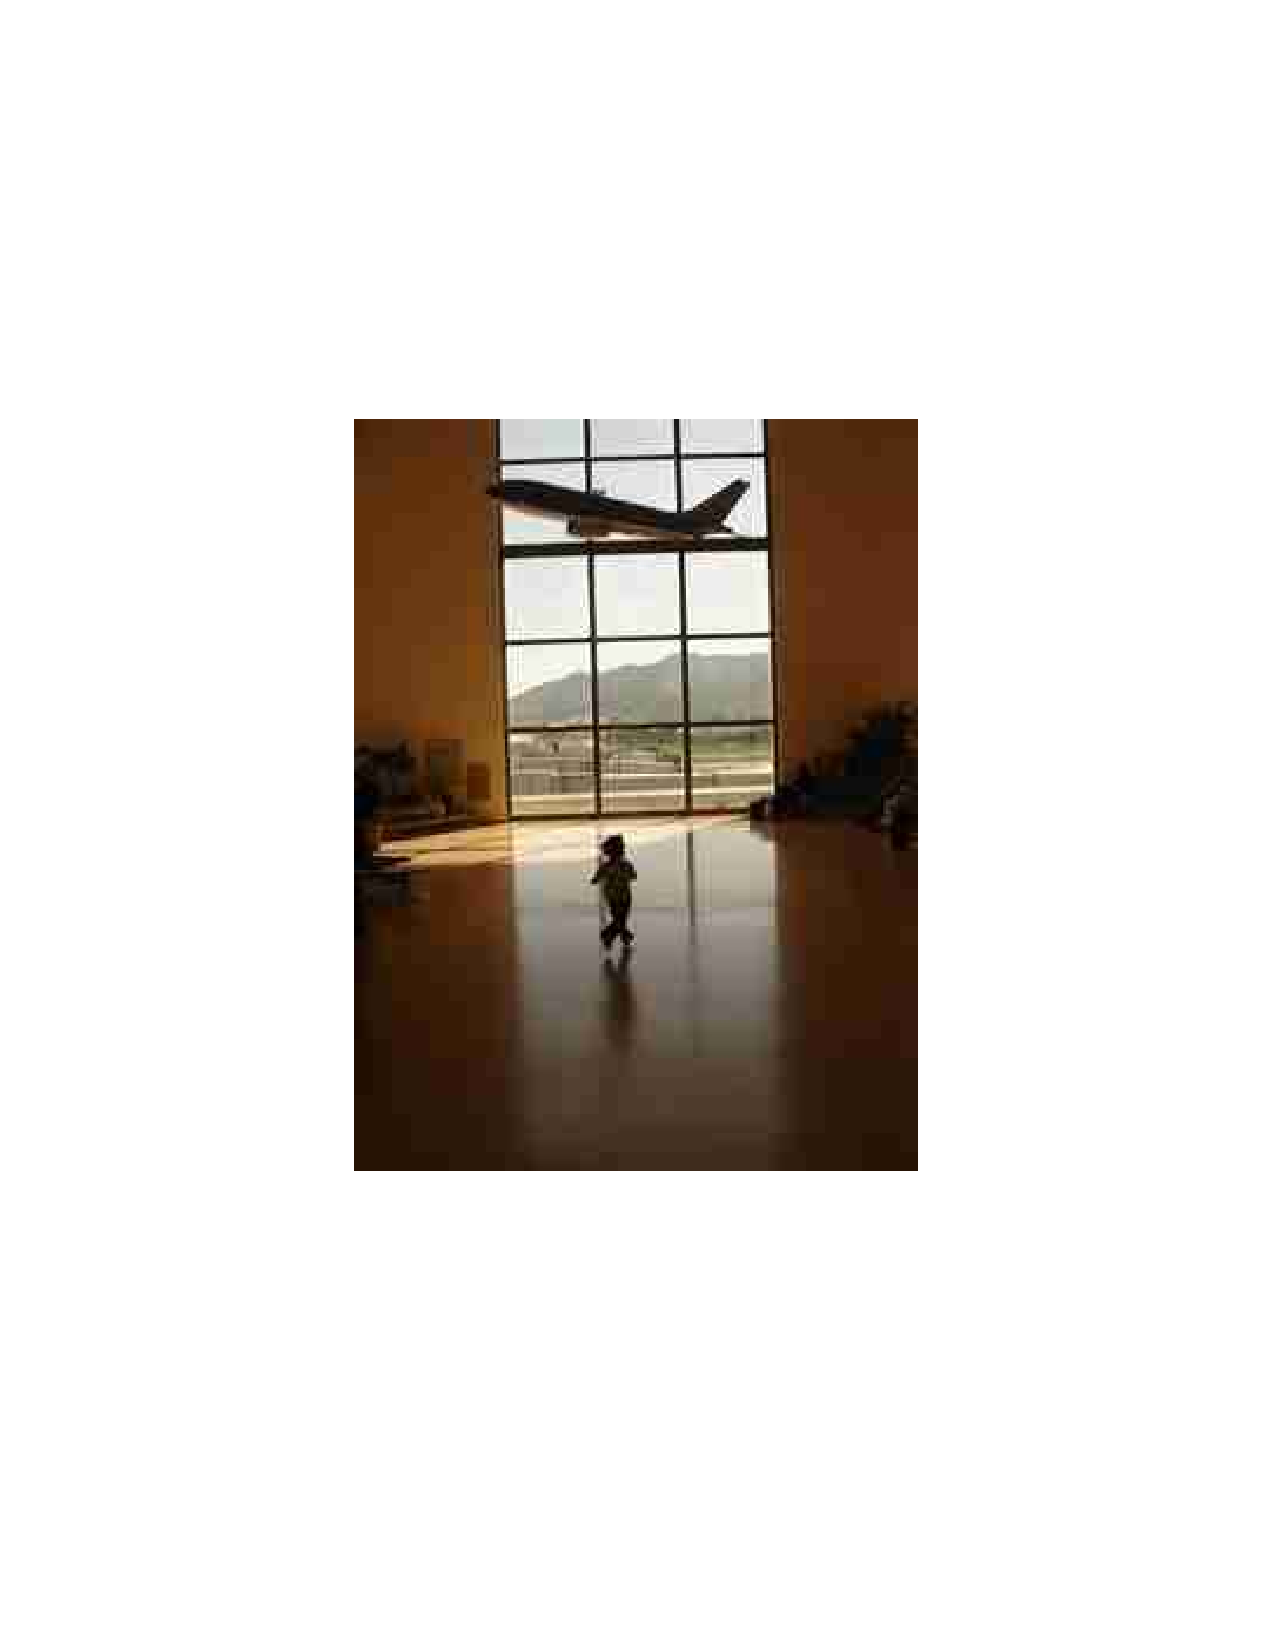
\includegraphics[trim=40mm 40mm 40mm 40mm,clip=true,width=0.45\linewidth]{images/airport_1.pdf} & 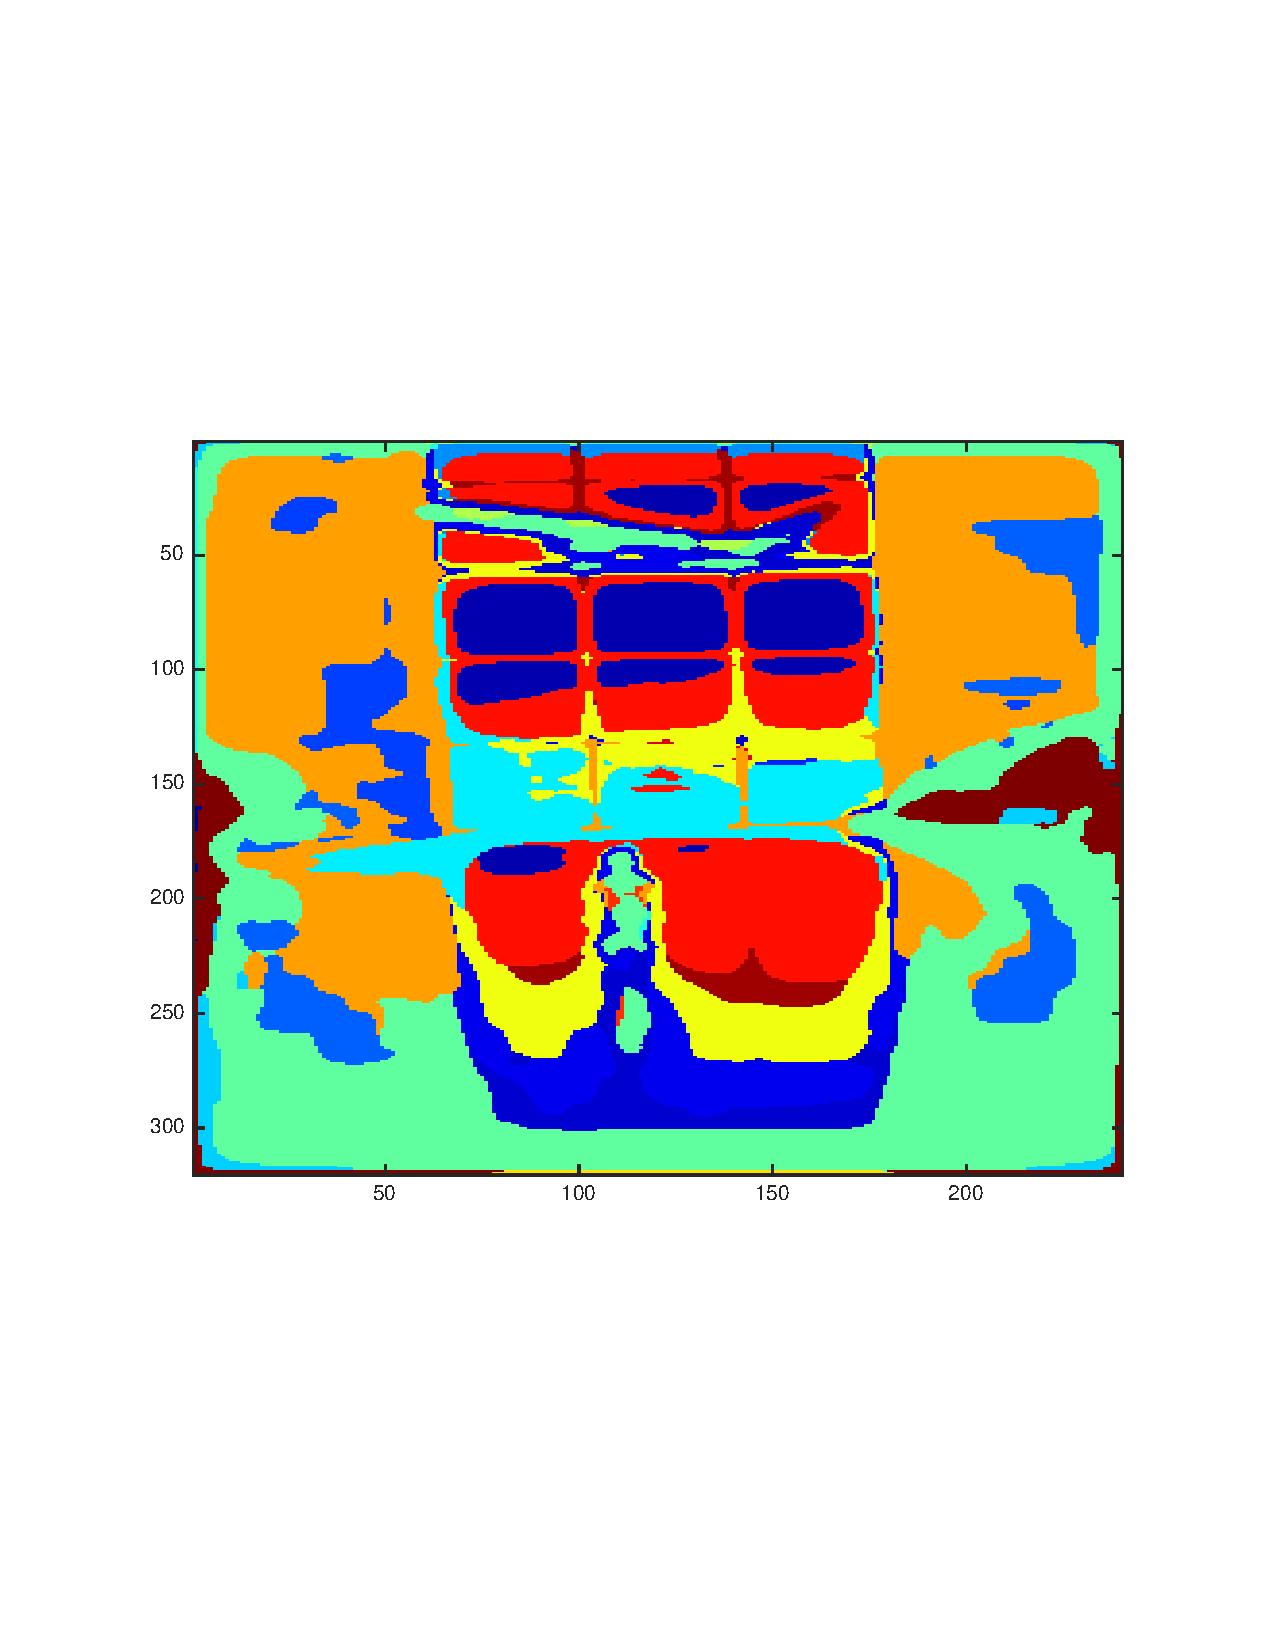
\includegraphics[trim=25mm 25mm 25mm 25mm,clip=true,width=0.45\linewidth]{images/airport_2.pdf} \\
  \hline
  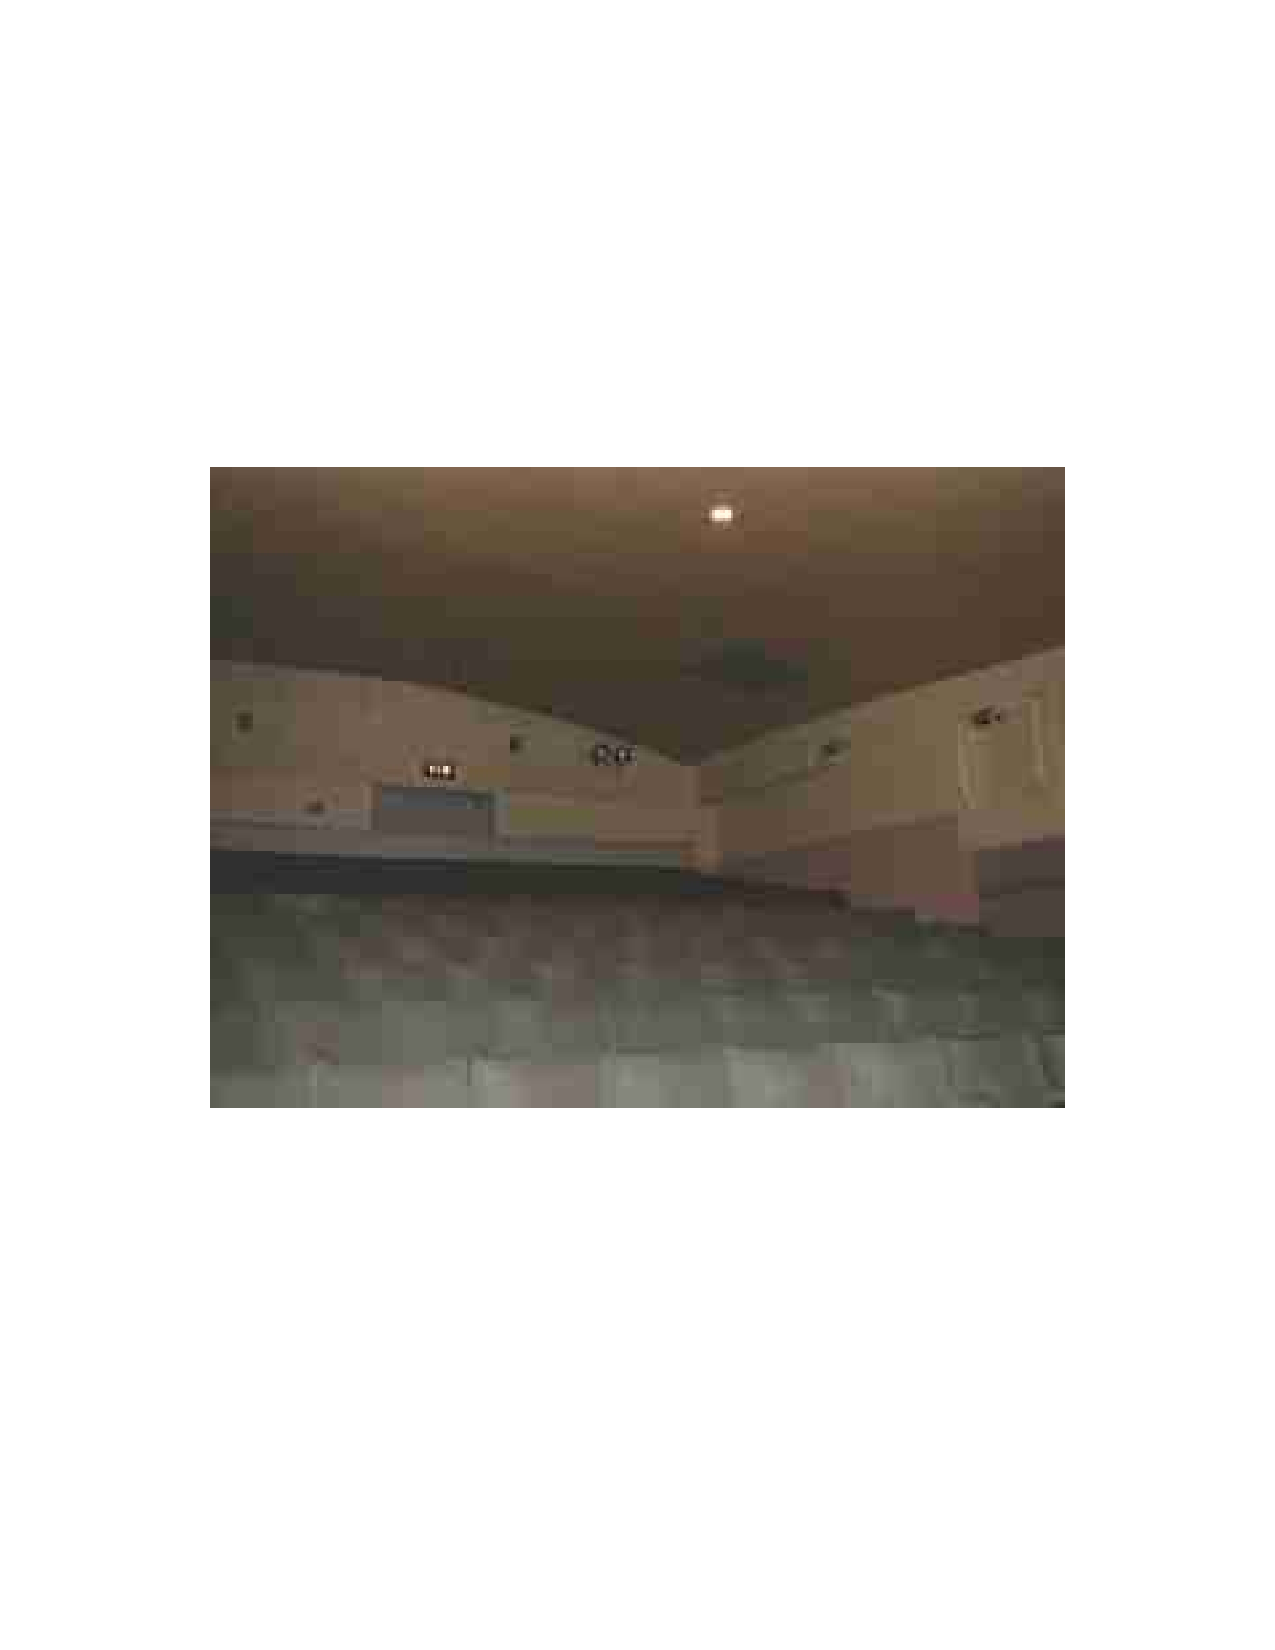
\includegraphics[trim=40mm 40mm 40mm 40mm,clip=true,width=0.45\linewidth]{images/auditorium_1.pdf} & 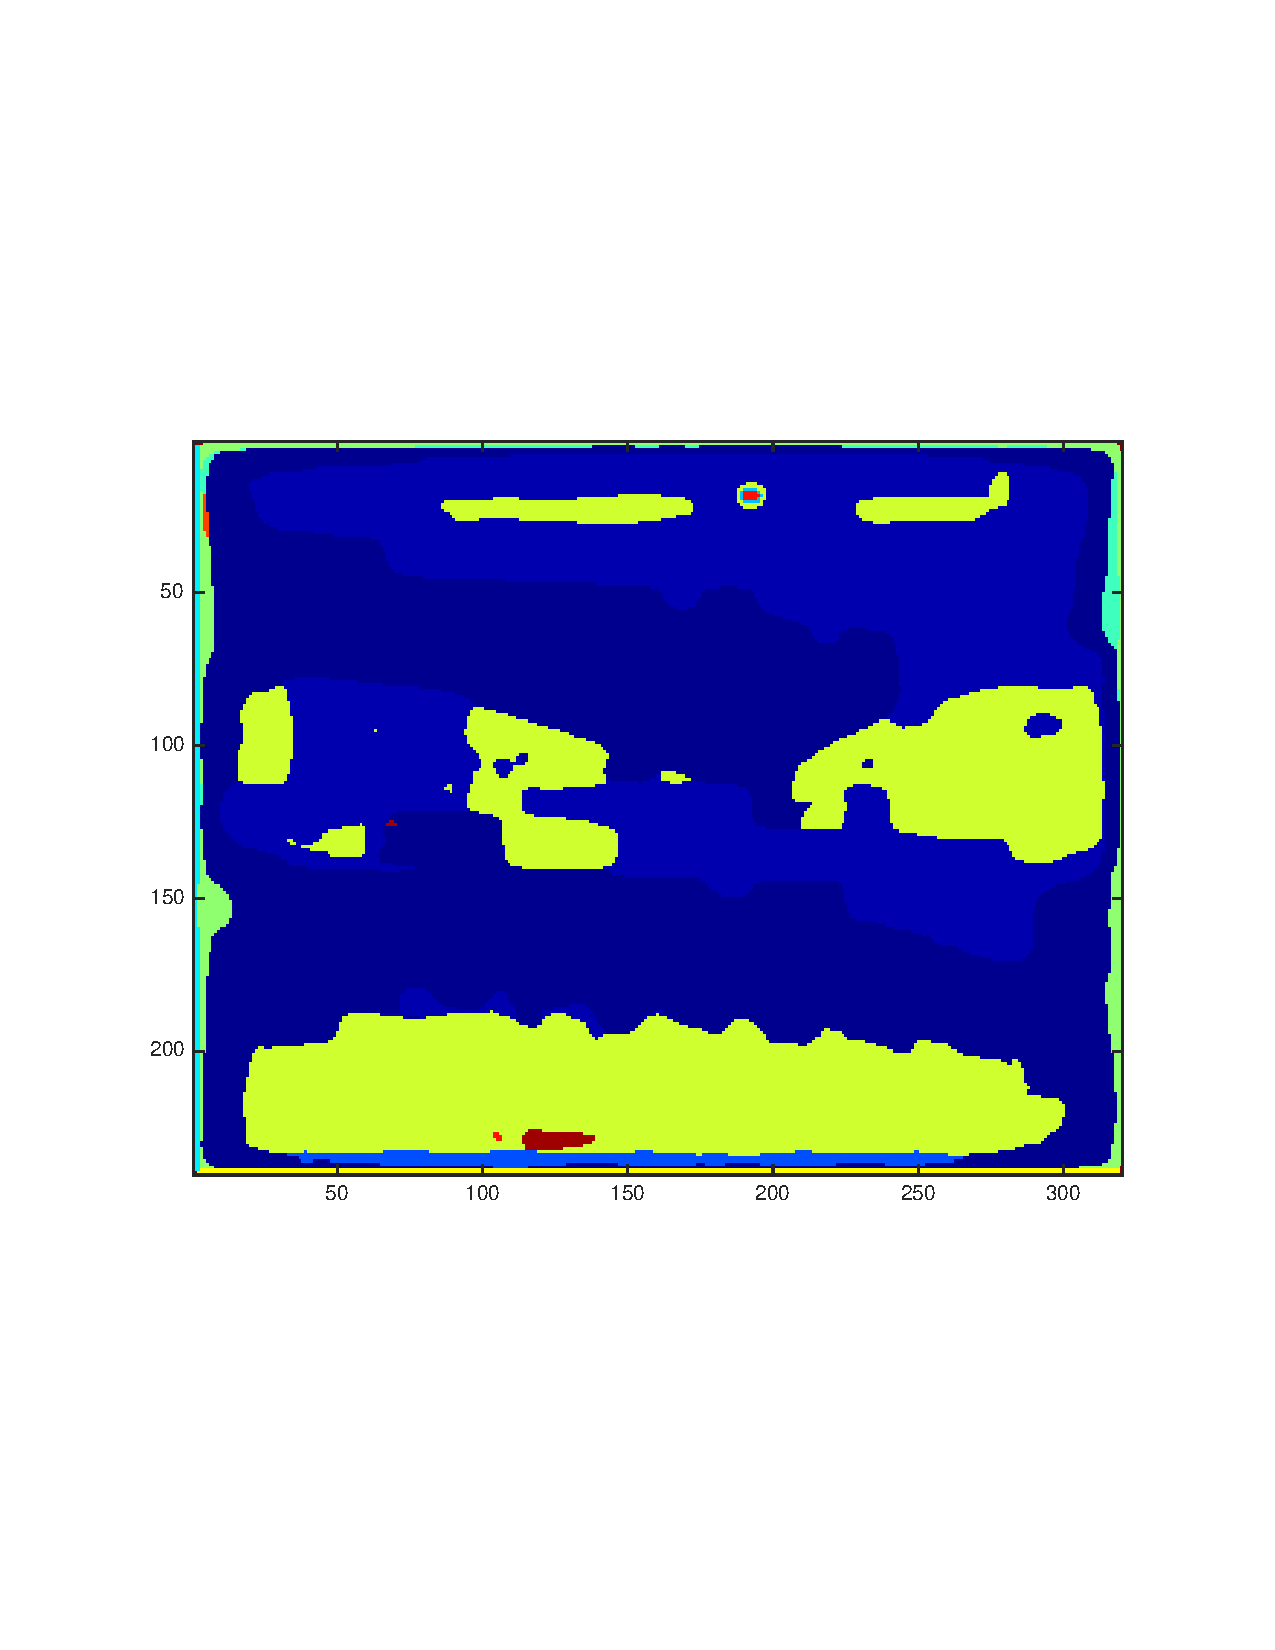
\includegraphics[trim=25mm 25mm 25mm 25mm,clip=true,width=0.45\linewidth]{images/auditorium_2.pdf} \\
  \hline
  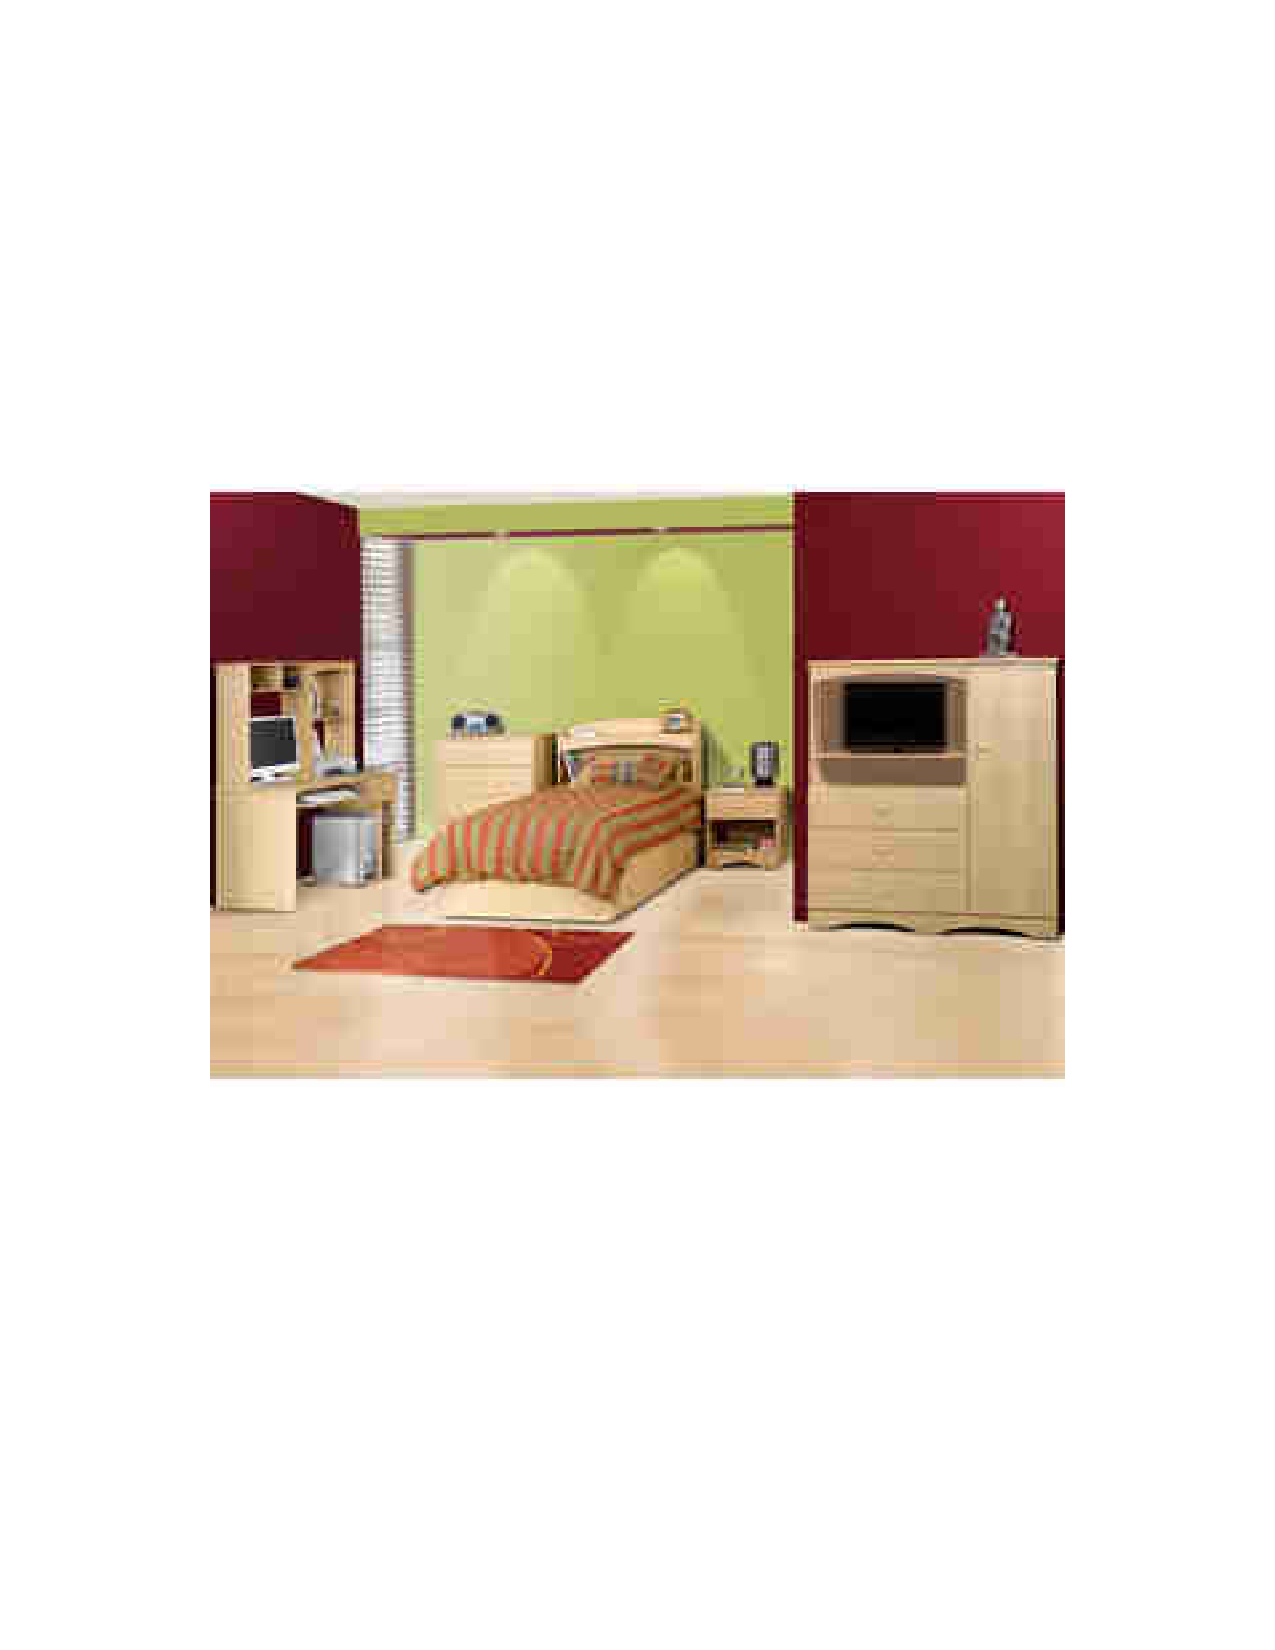
\includegraphics[trim=40mm 40mm 40mm 40mm,clip=true,width=0.45\linewidth]{images/bedroom_1.pdf} & 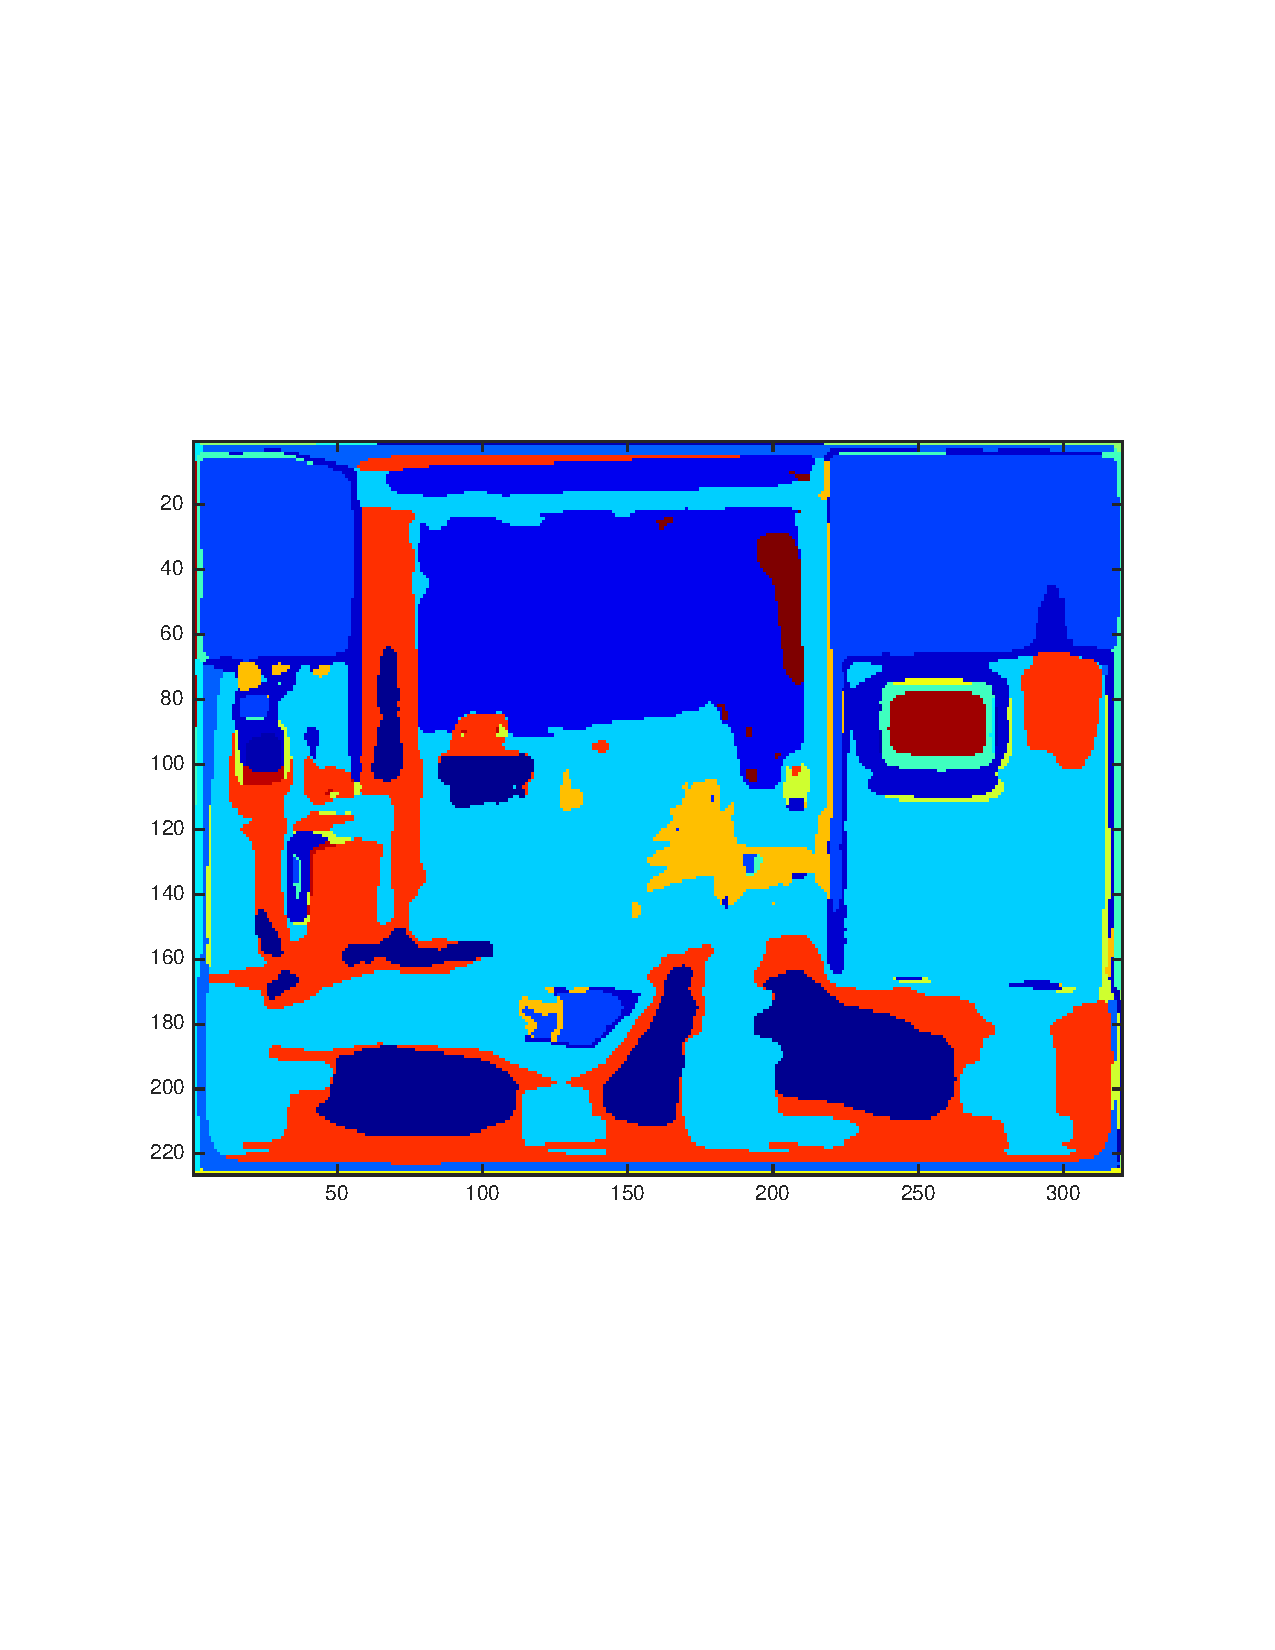
\includegraphics[trim=25mm 25mm 25mm 25mm,clip=true,width=0.45\linewidth]{images/bedroom_2.pdf} \\
  \hline
  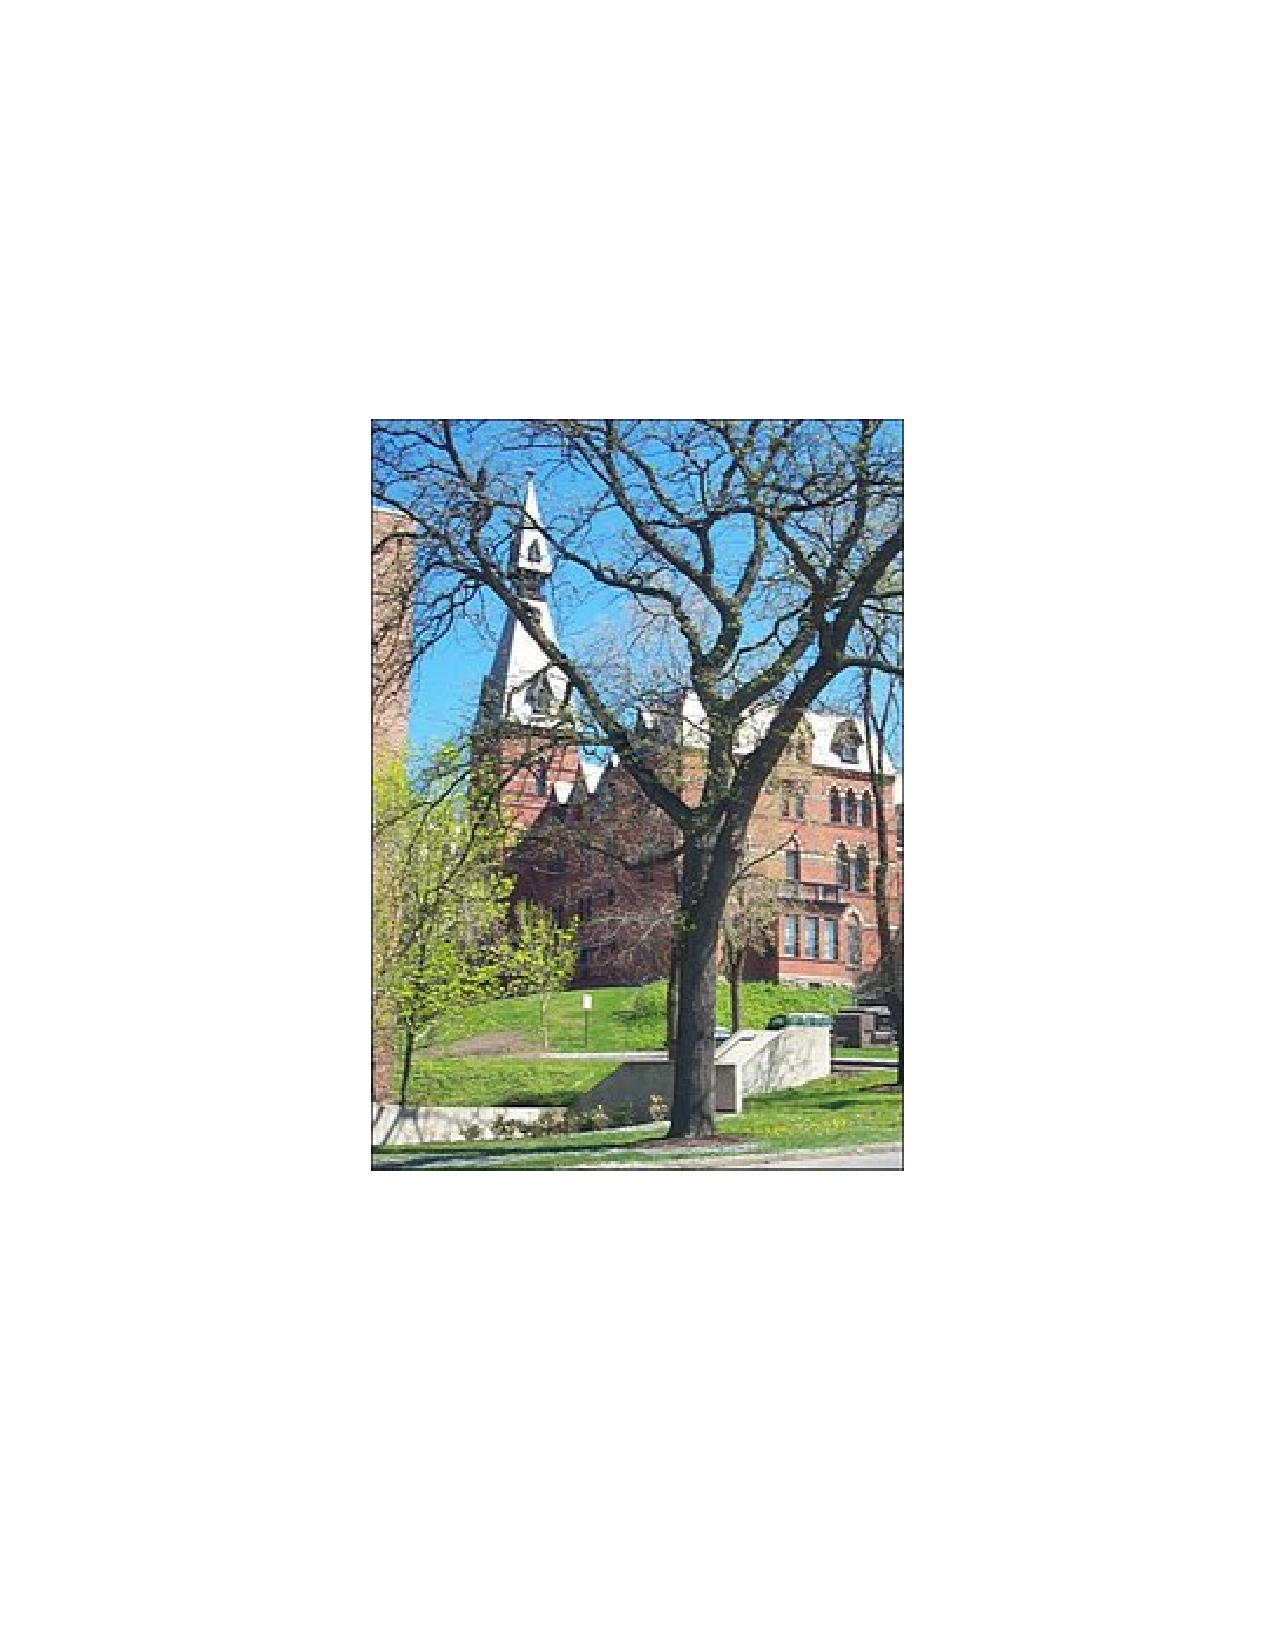
\includegraphics[trim=40mm 40mm 40mm 40mm,clip=true,width=0.45\linewidth]{images/campus_1.pdf} & 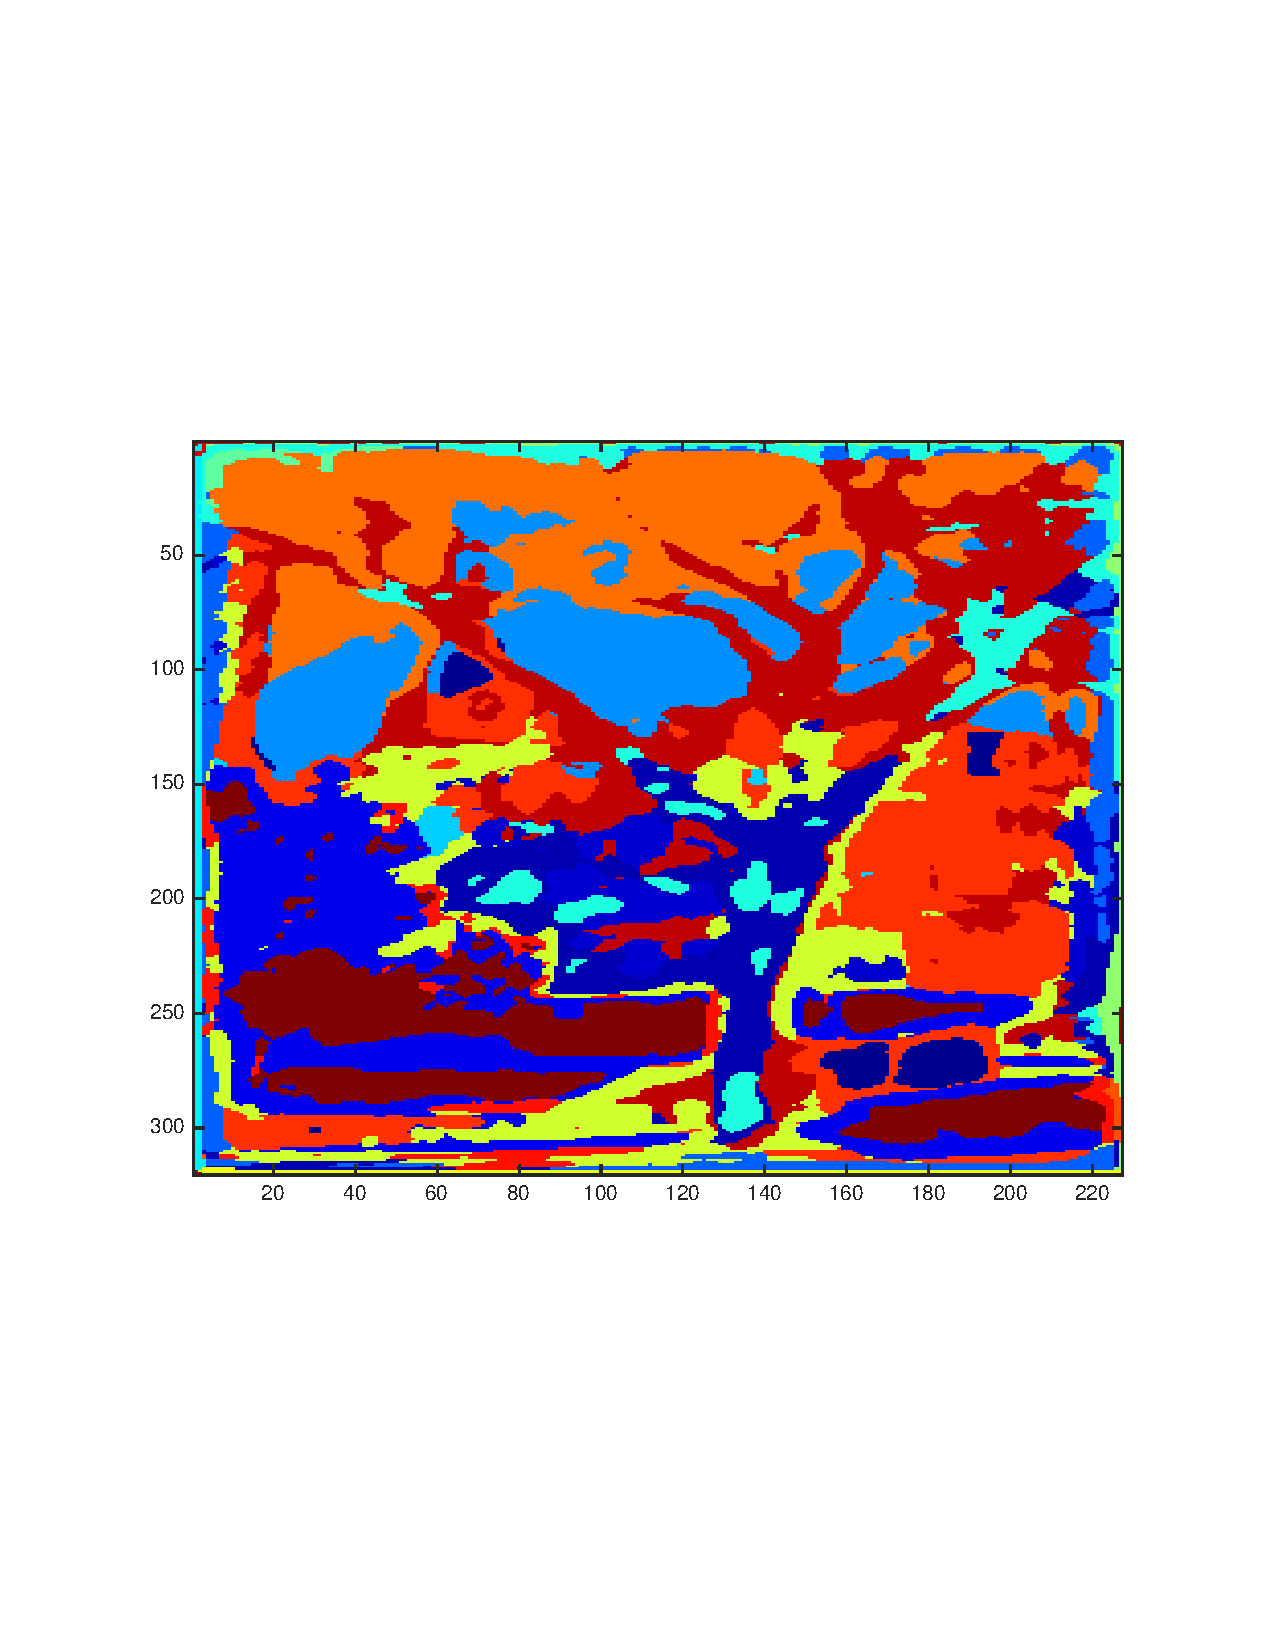
\includegraphics[trim=25mm 25mm 25mm 25mm,clip=true,width=0.45\linewidth]{images/campus_2.pdf} \\
  \hline
  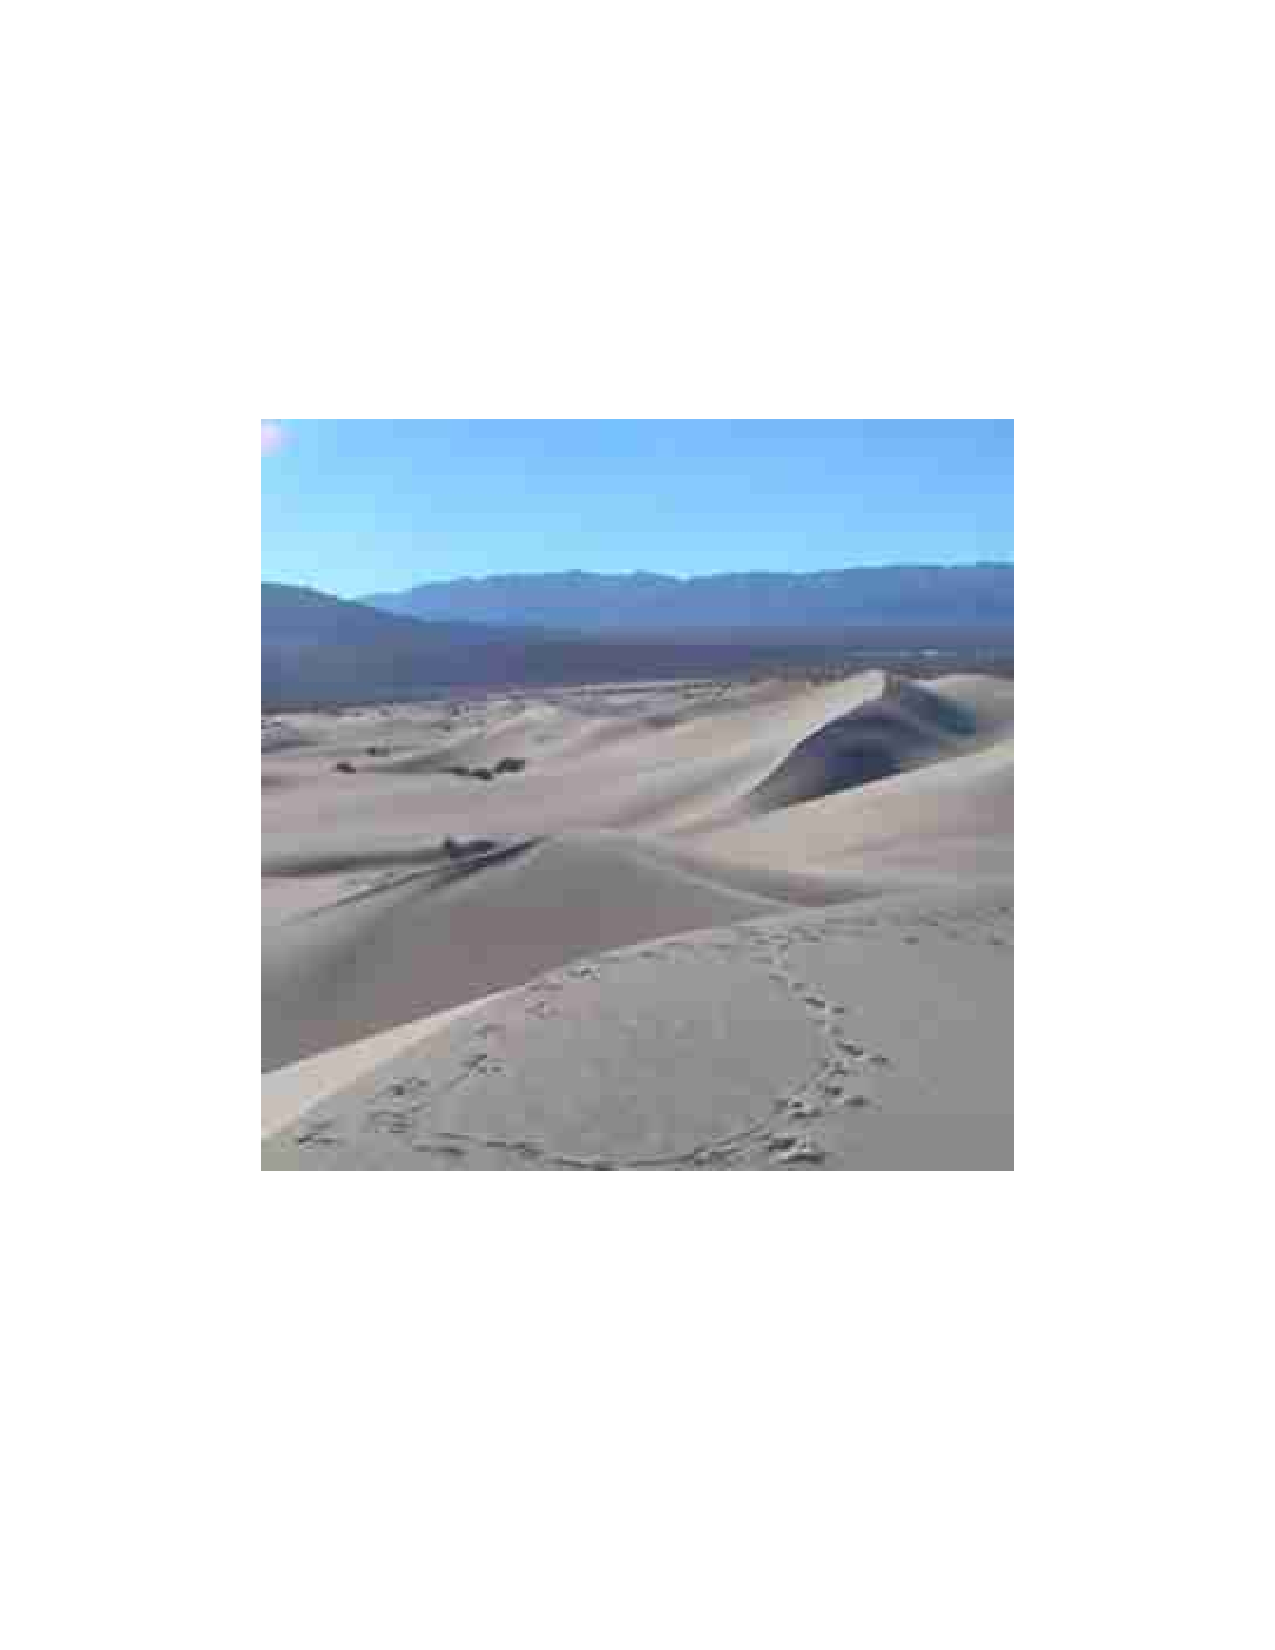
\includegraphics[trim=40mm 40mm 40mm 40mm,clip=true,width=0.45\linewidth]{images/desert_1.pdf} & 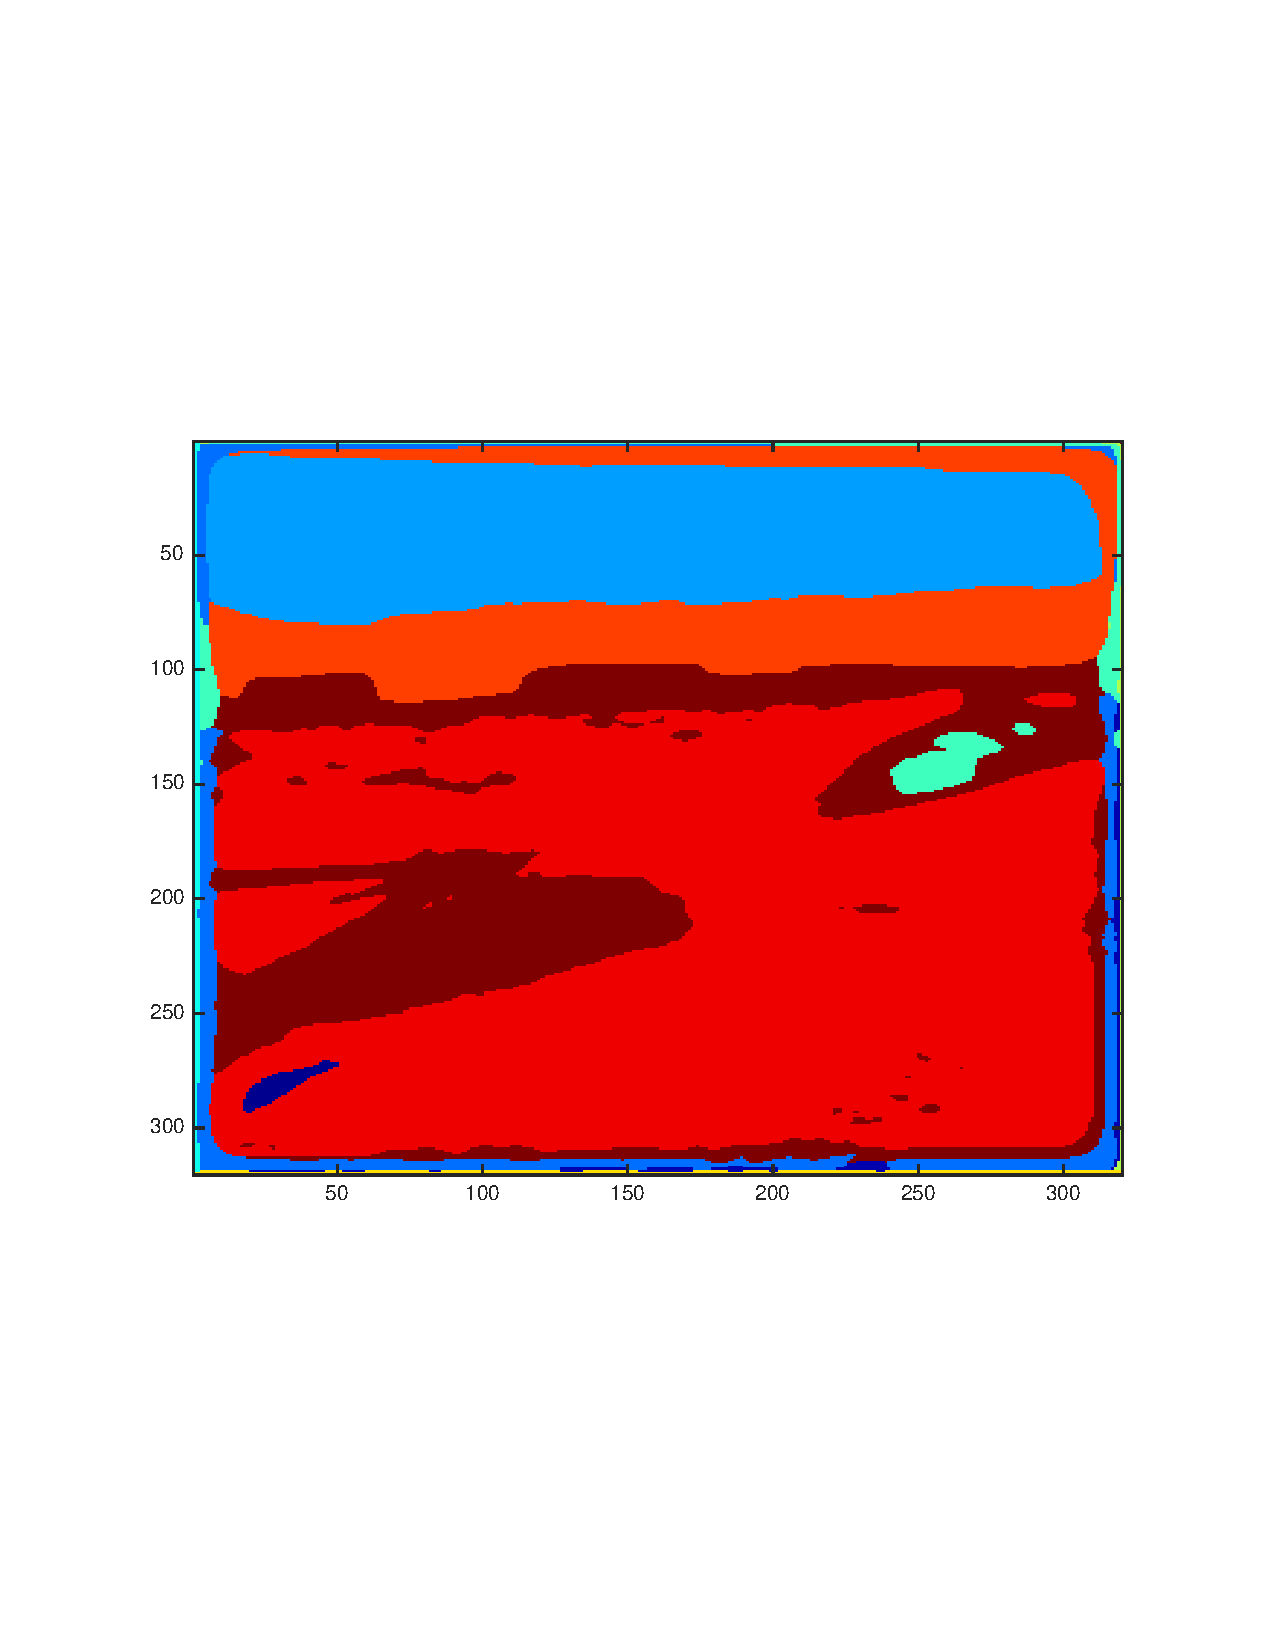
\includegraphics[trim=25mm 25mm 25mm 25mm,clip=true,width=0.45\linewidth]{images/desert_2.pdf} \\
  \hline
  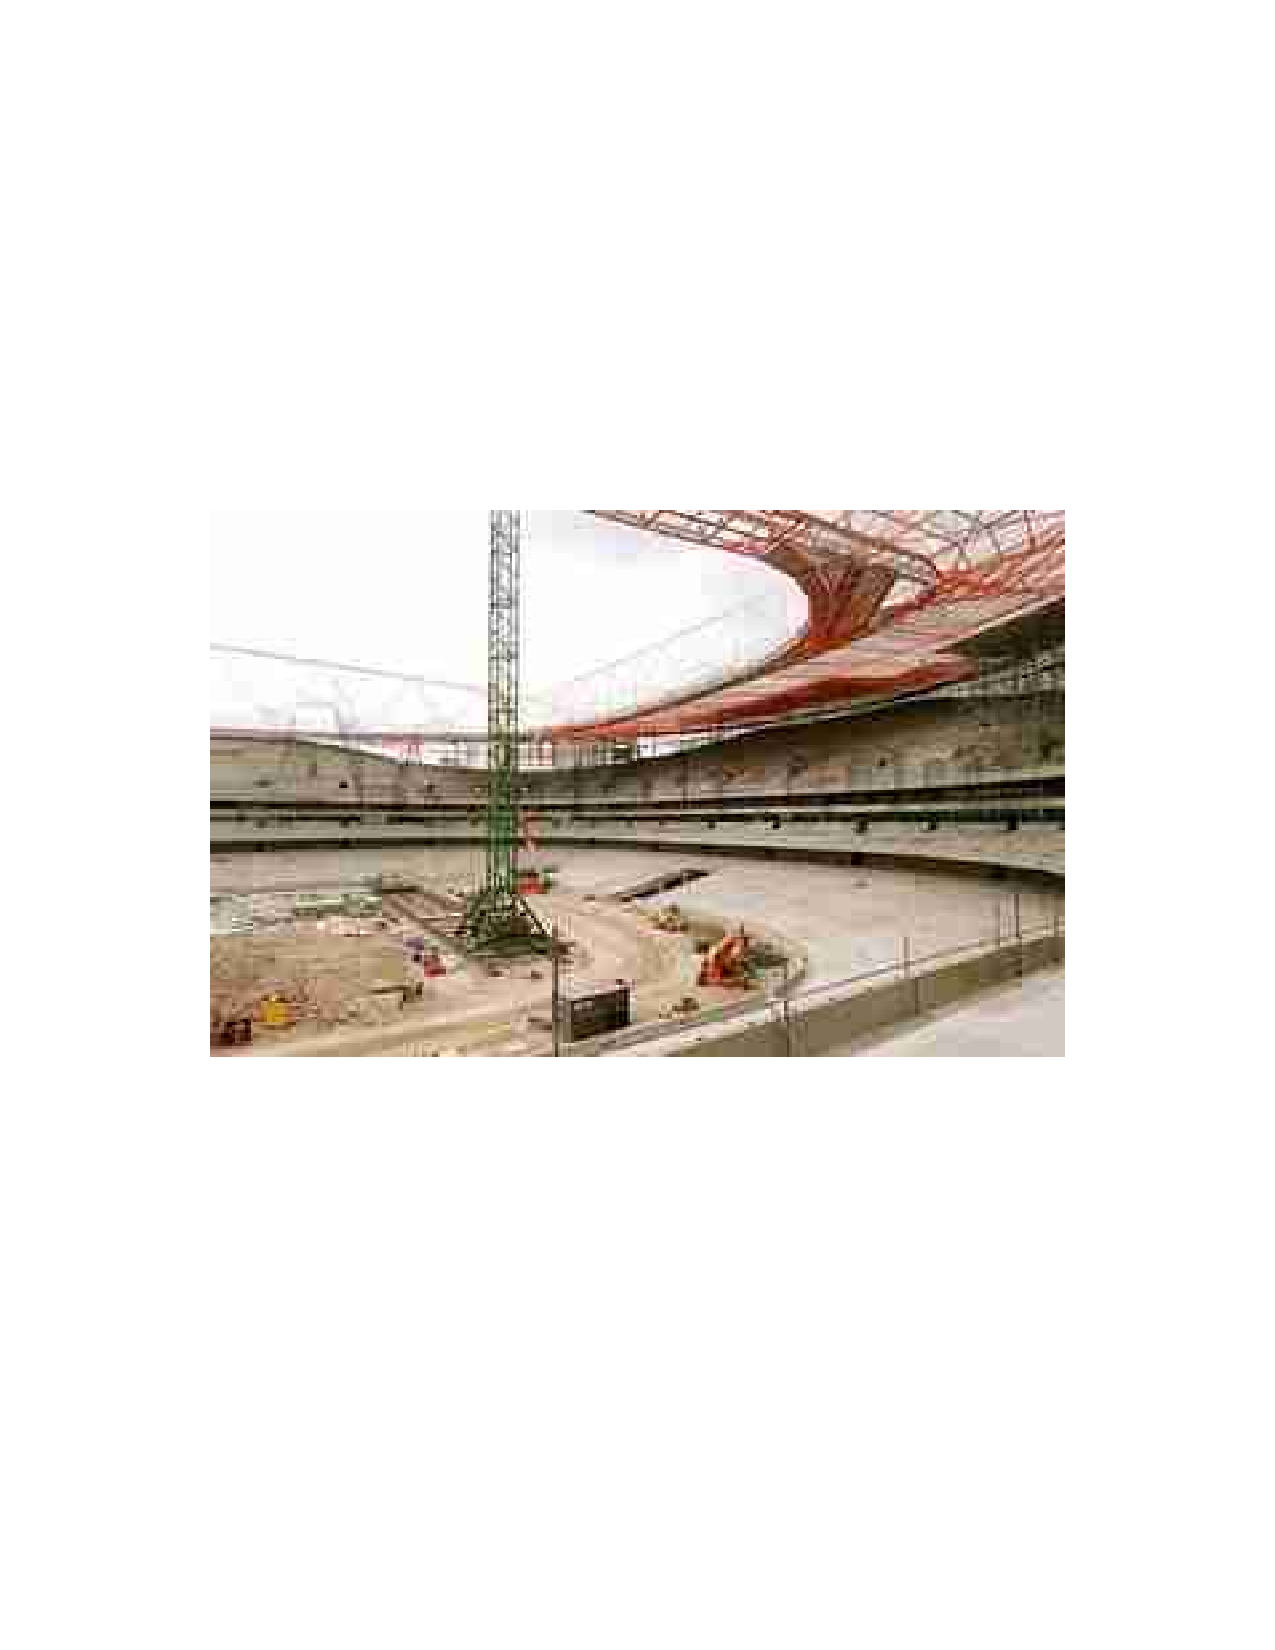
\includegraphics[trim=40mm 40mm 40mm 40mm,clip=true,width=0.45\linewidth]{images/stadium_1.pdf} & 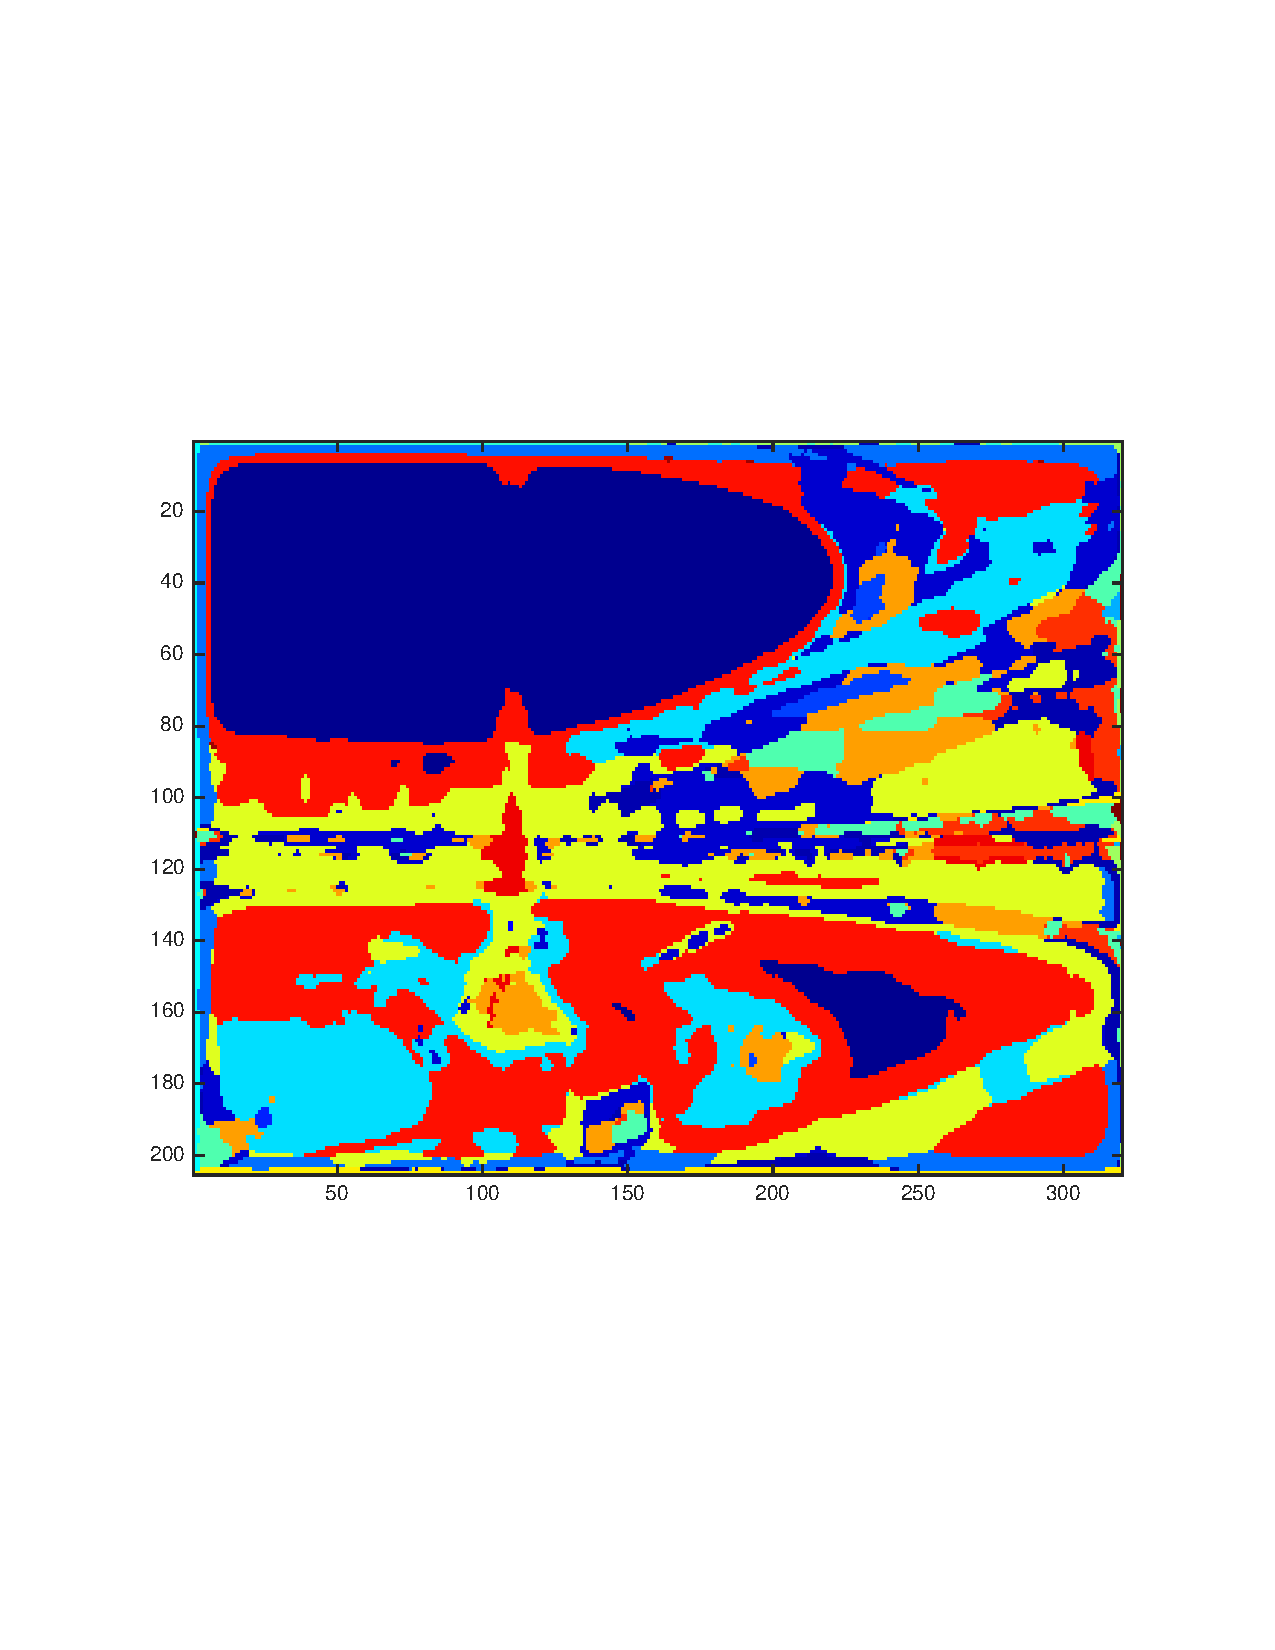
\includegraphics[trim=25mm 25mm 25mm 25mm,clip=true,width=0.45\linewidth]{images/stadium_2.pdf} \\
  \hline
  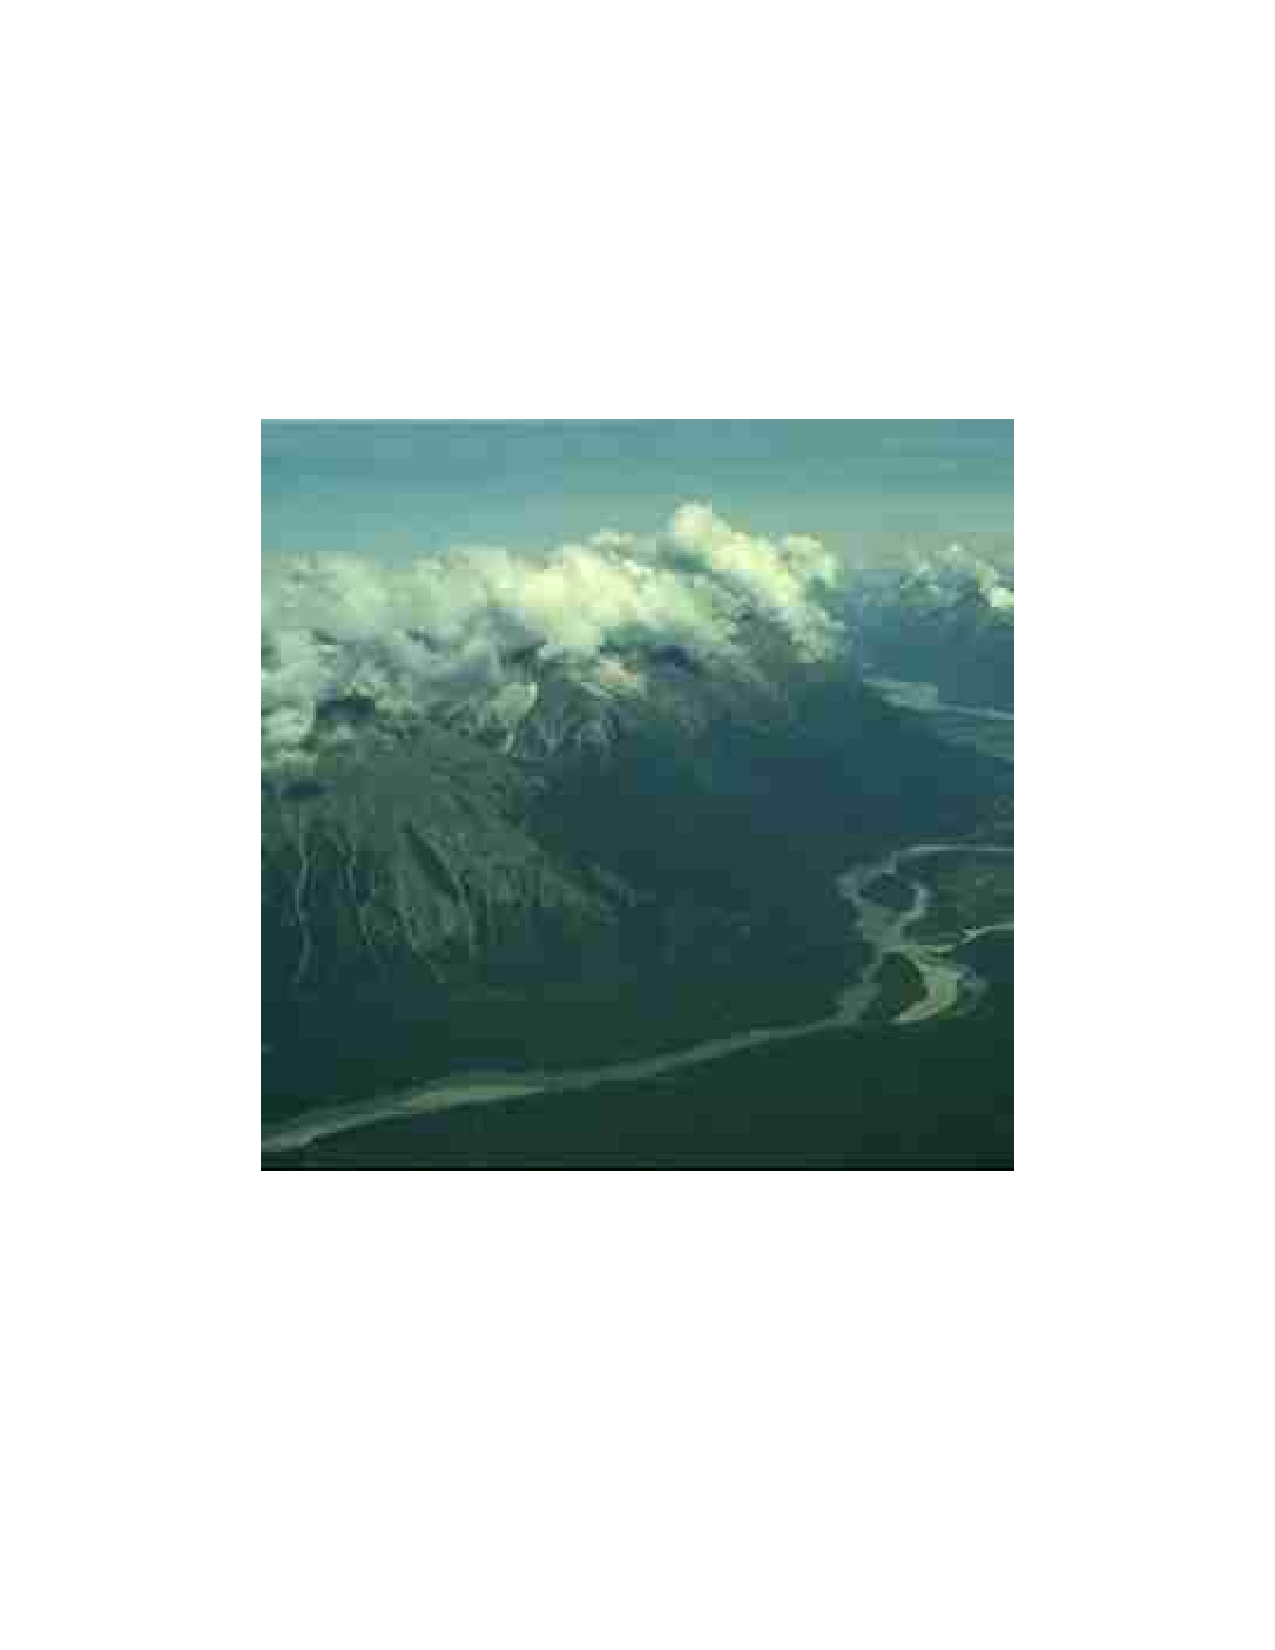
\includegraphics[trim=40mm 40mm 40mm 40mm,clip=true,width=0.45\linewidth]{images/landscape_1.pdf} & 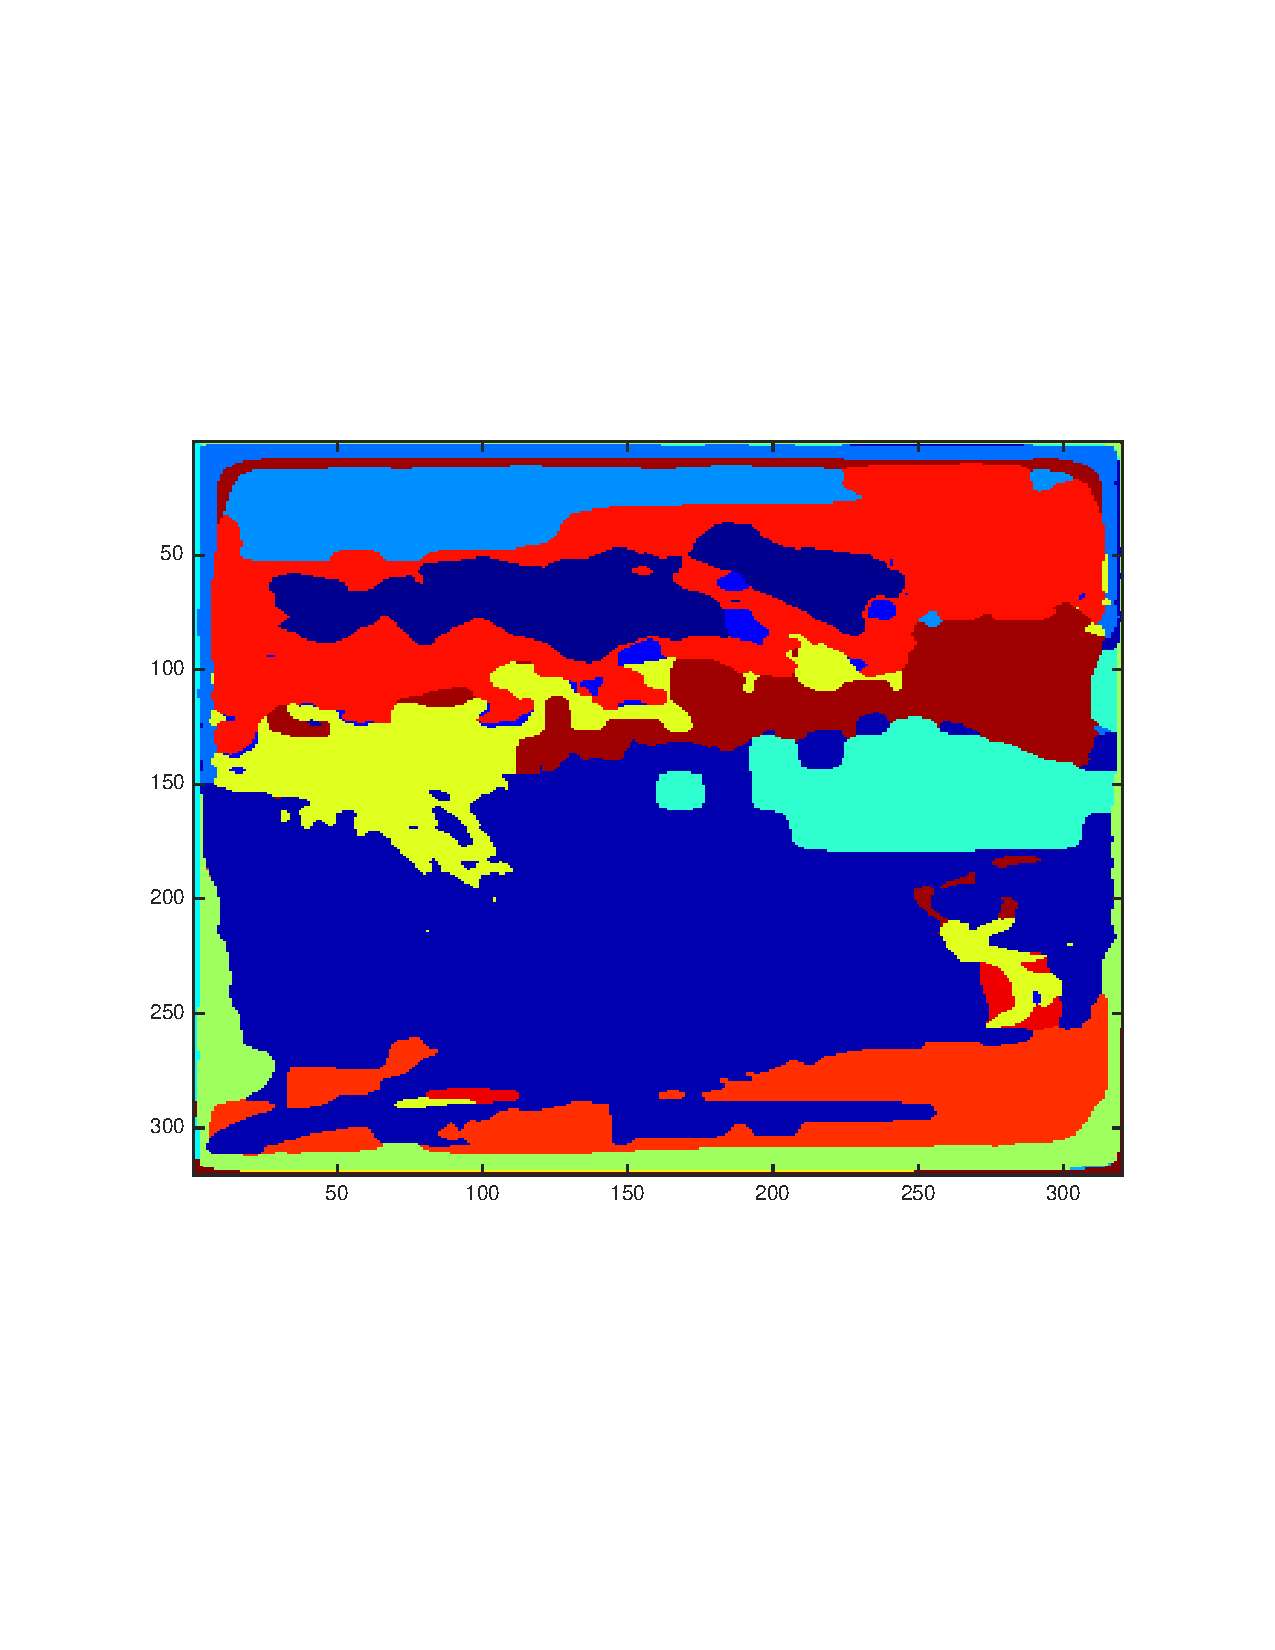
\includegraphics[trim=25mm 25mm 25mm 25mm,clip=true,width=0.45\linewidth]{images/landscape_2.pdf} \\
  \hline
  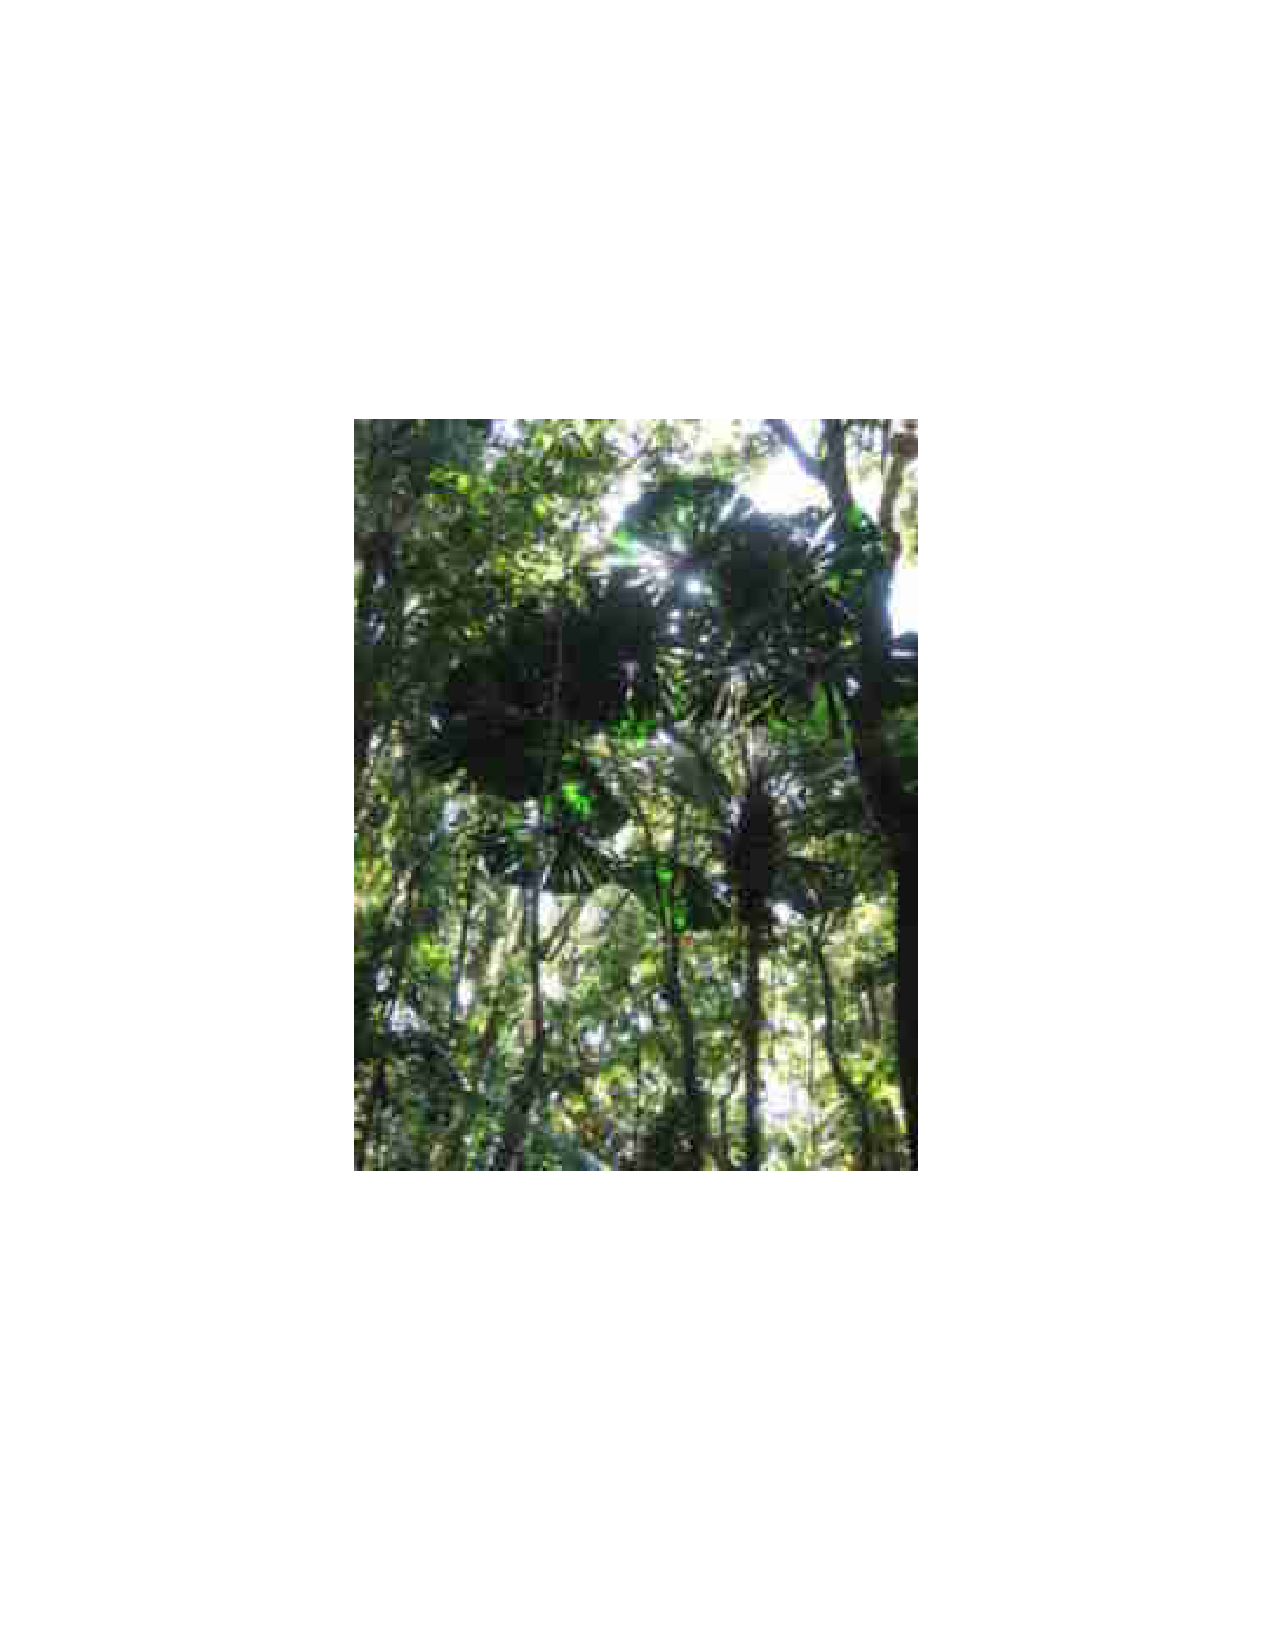
\includegraphics[trim=40mm 40mm 40mm 40mm,clip=true,width=0.45\linewidth]{images/rainforest_1.pdf} & 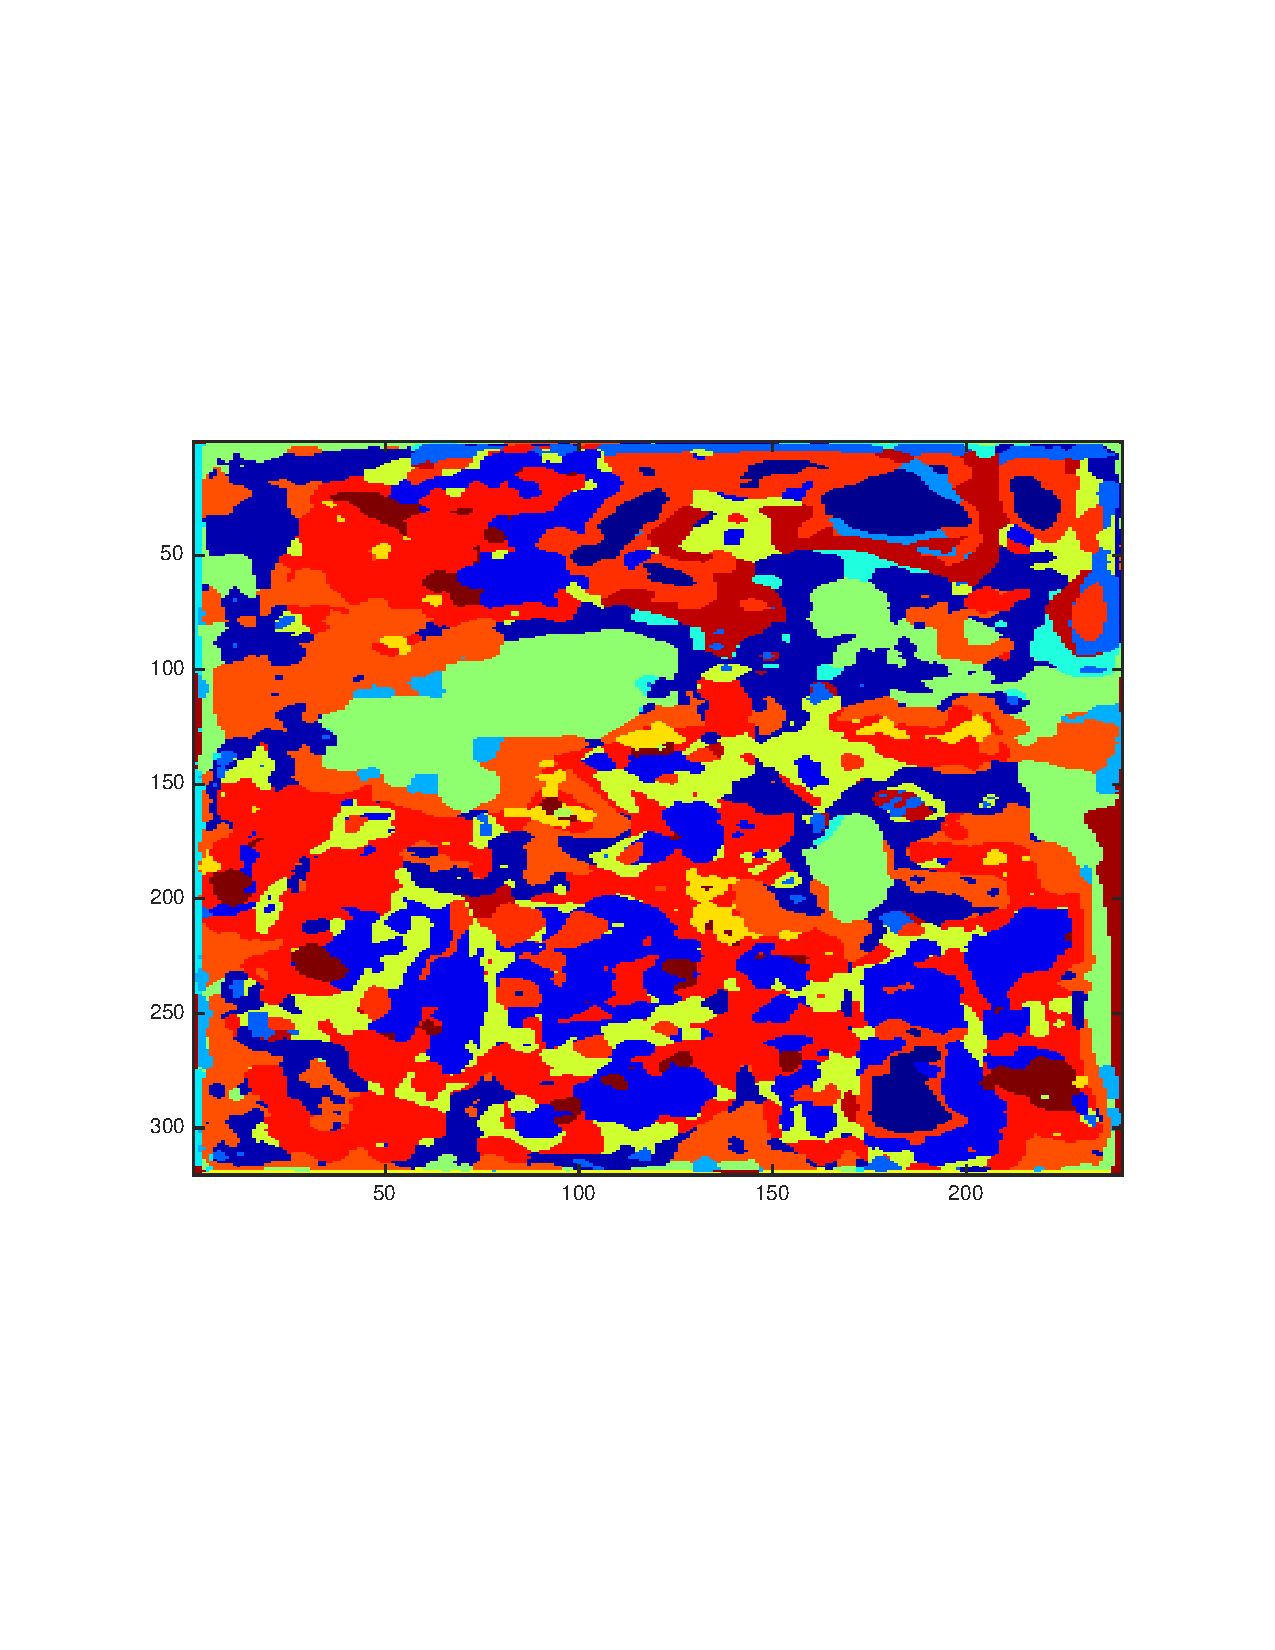
\includegraphics[trim=25mm 25mm 25mm 25mm,clip=true,width=0.45\linewidth]{images/rainforest_2.pdf} \\
  \hline
\caption{Output of \texttt{getVisualWords}}
\label{fig:visualwords}
\end{longtable}

\question{2.1}{getImageFeatures}

Included in \texttt{code/getImageFeatures.m} file

\question{2.2}{getImageFeaturesSPM}

Included in \texttt{code/getImageFeaturesSPM.m} file. It is coded using recursion for readability.

\question{2.3}{distanceToSet}

Included in \texttt{code/distanceToSet.m} file. It uses \emph{bsxfun} for improving performance.

\question{2.4}{buildRecognitionSystem}

Included in \texttt{code/buildRecognitionSystem.m} file

\question{2.5}{evaluateRecognitionSystem}

Included in \texttt{code/evaluateRecognitionSystem.m} file

The accuracy obtained was $51.88\%$. As we see later, this can be improved to around $61\%$ using the spearman distance metric and $K=19$ in the KNN classification.

The per class accuracy was as follows:

\begin{tabular}{|c |c |c |c |c |c |c |c|}
\hline
1 & 2 & 3 & 4 & 5 & 6 & 7 & 8 \\
\hline
airport & auditorium & bedroom & campus & desert & football stadium &landscape & rainforest \\
\hline
55  & 70   & 35   & 40  &  70   & 35  &  30   & 80 \\
\hline
\end{tabular}

The confusion matrix is as follows:

\begin{verbatim}
    11     3     3     2     0     3     1     3
     1    14     4     0     3     1     1     0
     4     1     7     1     1     0     0     0
     0     0     1     8     1     2     6     0
     1     2     5     2    14     3     3     1
     0     0     0     4     0     7     0     0
     0     0     0     3     1     3     6     0
     3     0     0     0     0     1     3    16
\end{verbatim}

\question{3.1}{Problems in Accuracy}

As we can see from the per class accuracy given above, classes with a significantly low accuracy are bedroom, landscape, and football stadium. The highest cross-category number in the confusion matrix is 
6 for landscape-campus pair, indicating that many landscape photos are getting confused as campuses. Below are the mistakes that were reported in the classification. The first mistake in each category is in bold font and accompanied by the corresponding image.

{\bf Mistake on airport/sun\_aerinlrdodkqnypz.jpg classified as auditorium (very plausible) \\}
\begin{figure}
\centering
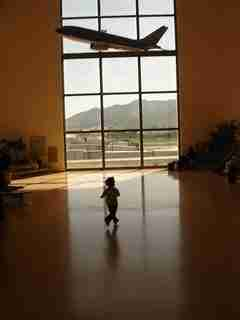
\includegraphics[width=0.5\linewidth]{../dat/airport/sun_aerinlrdodkqnypz.jpg}
\end{figure}
Mistake on airport/sun\_aetygbcukodnyxkl.jpg classified as bedroom \\
Mistake on airport/sun\_aevitxnlfjzhdnti.jpg classified as bedroom \\
Mistake on airport/sun\_aevyxplabnmalatl.jpg classified as bedroom \\
Mistake on airport/sun\_aexdiixgtdqjzjpl.jpg classified as rainforest \\
Mistake on airport/sun\_aexxslabfmbsumkp.jpg classified as rainforest \\
Mistake on airport/sun\_aeyqkdhbapysbwbv.jpg classified as desert \\
Mistake on airport/sun\_afacqjwmeipxtsdu.jpg classified as rainforest \\
Mistake on airport/sun\_afbxsdfksjhcunpb.jpg classified as bedroom \\
{\bf Mistake on auditorium/sun\_aadrvlcduunrbpul.jpg classified as airport \\}
\begin{figure}
\centering
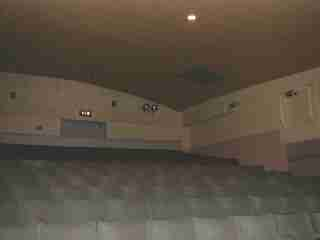
\includegraphics[width=0.5\linewidth]{../dat/auditorium/sun_aadrvlcduunrbpul.jpg}
\end{figure}
Mistake on auditorium/sun\_abjkjhdyminvtxsm.jpg classified as airport \\
Mistake on auditorium/sun\_abnptawlxcjefrmi.jpg classified as airport \\
Mistake on auditorium/sun\_abufkgwvilfzdqys.jpg classified as desert \\
Mistake on auditorium/sun\_acsdhbbsybcyxnel.jpg classified as bedroom \\
Mistake on auditorium/sun\_acsxxurtqimfqbog.jpg classified as desert \\
{\bf Mistake on bedroom/sun\_aafesxmciavqmkxw.jpg classified as campus \\}
\begin{figure}
\centering
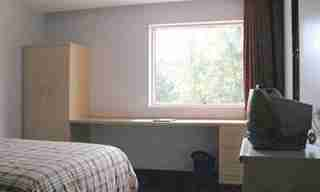
\includegraphics[width=0.5\linewidth]{../dat/bedroom/sun_aafesxmciavqmkxw.jpg}
\end{figure}
Mistake on bedroom/sun\_aaoqcwcewjvnfeps.jpg classified as auditorium \\
Mistake on bedroom/sun\_aaprepyzloaivblt.jpg classified as desert \\
Mistake on bedroom/sun\_aarvhntgsdfxgmmb.jpg classified as auditorium \\
Mistake on bedroom/sun\_aauzqebrqbqgzece.jpg classified as airport \\
Mistake on bedroom/sun\_aaxfqfzrjwrlfwuf.jpg classified as auditorium \\
Mistake on bedroom/sun\_aaxspwgpppcwlqht.jpg classified as airport \\
Mistake on bedroom/sun\_aazccosvjonbhrff.jpg classified as desert \\
Mistake on bedroom/sun\_abfukgjexiwonarv.jpg classified as auditorium \\
Mistake on bedroom/sun\_abgsudgeaejqbwtn.jpg classified as desert \\
Mistake on bedroom/sun\_abkzhpaluuxwcfdk.jpg classified as desert \\
Mistake on bedroom/sun\_abpmyykpuijkvxbq.jpg classified as desert \\
Mistake on bedroom/sun\_absevjzddeawnmko.jpg classified as airport \\
{\bf Mistake on campus/sun\_abpxvcuxhqldcvln.jpg classified as football\_stadium \\}
\begin{figure}
\centering
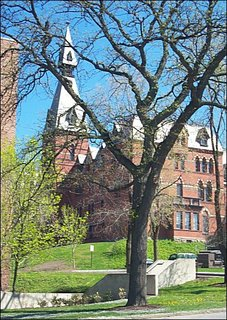
\includegraphics[width=0.5\linewidth]{../dat/campus/sun_abpxvcuxhqldcvln.jpg}
\end{figure}
Mistake on campus/sun\_abslhphpiejdjmpz.jpg classified as football\_stadium \\
Mistake on campus/sun\_abwbqwhaqxskvyat.jpg classified as football\_stadium \\
Mistake on campus/sun\_aczmgnjjiykpqyts.jpg classified as bedroom \\
Mistake on campus/sun\_adiqdyqsqarvtact.jpg classified as landscape \\
Mistake on campus/sun\_agjdyybkyzxpqips.jpg classified as desert \\
Mistake on campus/sun\_agruqaefvrvumwod.jpg classified as landscape \\
Mistake on campus/sun\_ahdehpqieqxgehgy.jpg classified as landscape \\
Mistake on campus/sun\_ahprylpgnmgqiyuz.jpg classified as airport \\
Mistake on campus/sun\_ahsxqcejwxphkyih.jpg classified as desert \\
Mistake on campus/sun\_ajrlkrwvvsenzpyt.jpg classified as airport \\
Mistake on campus/sun\_akguesajnqnoyszx.jpg classified as football\_stadium \\
{\bf Mistake on desert/sun\_acztaebqvjaggqyh.jpg classified as auditorium \\}
\begin{figure}
\centering
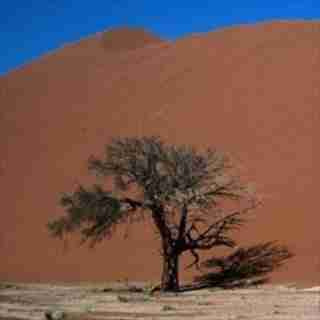
\includegraphics[width=0.5\linewidth]{../dat/desert/sun_acztaebqvjaggqyh.jpg}
\end{figure}
Mistake on desert/sun\_adbymuzeqfdwlerv.jpg classified as auditorium \\
Mistake on desert/sun\_aggpnmjzyopfvkxd.jpg classified as auditorium \\
Mistake on desert/sun\_aiatoxvclffgxjts.jpg classified as campus \\
Mistake on desert/sun\_aijjkofxcvbaoewh.jpg classified as bedroom \\
Mistake on desert/sun\_aimopcdnurqckhhc.jpg classified as landscape \\
{\bf Mistake on football\_stadium/sun\_aahvylyxdakauexd.jpg classified as airport \\}
\begin{figure}
\centering
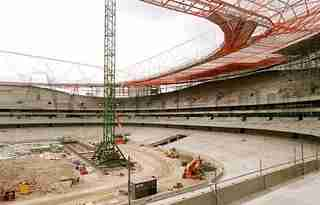
\includegraphics[width=0.5\linewidth]{../dat/football_stadium/sun_aahvylyxdakauexd.jpg}
\end{figure}
Mistake on football\_stadium/sun\_abcyqxcuxdpbmgkn.jpg classified as airport \\
Mistake on football\_stadium/sun\_ajersoqqetrcgtkd.jpg classified as landscape \\
Mistake on football\_stadium/sun\_akgsvnkdoawntqoj.jpg classified as desert \\
Mistake on football\_stadium/sun\_aliwekqtpmatjrfk.jpg classified as campus \\
Mistake on football\_stadium/sun\_ampjzbnckfgejpsl.jpg classified as desert \\
Mistake on football\_stadium/sun\_anzijotshmbcendh.jpg classified as auditorium \\
Mistake on football\_stadium/sun\_apugcjcmszqqdwxw.jpg classified as rainforest \\
Mistake on football\_stadium/sun\_arjxmegqfeavsozz.jpg classified as landscape \\
Mistake on football\_stadium/sun\_asqkycmnpaeazziw.jpg classified as landscape \\
Mistake on football\_stadium/sun\_atcbgeektodzgvyu.jpg classified as airport \\
Mistake on football\_stadium/sun\_ayhhjsfptncuadib.jpg classified as desert \\
Mistake on football\_stadium/sun\_bauycdcdmruicjvw.jpg classified as campus \\
{\bf Mistake on landscape/sun\_absddryibdeqqvqf.jpg classified as campus \\}
\begin{figure}
\centering
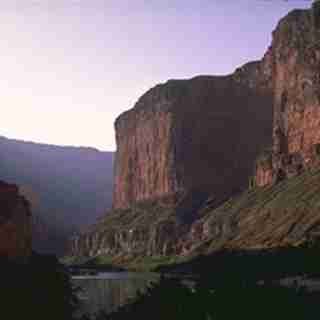
\includegraphics[width=0.5\linewidth]{../dat/landscape/sun_absddryibdeqqvqf.jpg}
\end{figure}
Mistake on landscape/sun\_abvvlqznpdszhjnh.jpg classified as rainforest \\
Mistake on landscape/sun\_adbbdotjpvckknnr.jpg classified as campus \\
Mistake on landscape/sun\_adbtakwewxdagnxp.jpg classified as campus \\
Mistake on landscape/sun\_adqxdqlbhuiagrqt.jpg classified as rainforest \\
Mistake on landscape/sun\_aduxybjjxgfhwggu.jpg classified as rainforest \\
Mistake on landscape/sun\_aefbezeufxvlpxgd.jpg classified as desert \\
Mistake on landscape/sun\_aeldkedqeopyedlo.jpg classified as campus \\
Mistake on landscape/sun\_aewjouuoxozhzmsx.jpg classified as auditorium \\
Mistake on landscape/sun\_afhhnevciblqzhjp.jpg classified as campus \\
Mistake on landscape/sun\_afiznkgdkgugndcx.jpg classified as desert \\
Mistake on landscape/sun\_afjdogbpwckftyfl.jpg classified as desert \\
Mistake on landscape/sun\_afliehgwaoiynwcw.jpg classified as airport \\
Mistake on landscape/sun\_ahekiunfgsyehcbg.jpg classified as campus \\
{\bf Mistake on rainforest/sun\_aalbylumieujfxrc.jpg classified as desert \\}
\begin{figure}
\centering
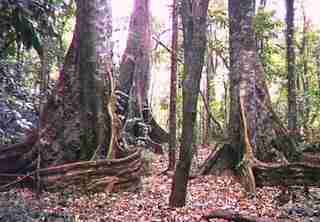
\includegraphics[width=0.5\linewidth]{../dat/rainforest/sun_aalbylumieujfxrc.jpg}
\end{figure}
Mistake on rainforest/sun\_aangkajdydimnqru.jpg classified as airport \\
Mistake on rainforest/sun\_abafooecdwxfwlob.jpg classified as airport \\
Mistake on rainforest/sun\_abuyerbrwfrujntz.jpg classified as airport \\

\question{3.2}{Improvements in Accuracy}

To improve accuracy, I considered varying the number of neighbors in the KNN classification and the distance metric used to calculate the nearest neighbors. This made a huge difference to the accuracy of the algorithm. The results are shown in figure (\ref{fig:accuracy}); please zoom if the image is not clear. The X axis is the number of nearest neighbors used in the KNN classification, and the Y axis shows the corresponding accuracy. The four curves correspond to four distance metrics - euclidean distance, cityblock distance (also known as manhattan distance), cosine distance, and spearman correlation distance. As we can see from the figure, the accuracy results from the spearman distance metric uniformly dominate other distance metrics at all $K$. Using spearman distance and $K=19$, we get the best accuracy of $61.25\%$. When $K>6$, spearman distance metric generally gives good accuracy results between $58.75\%$ and $61.25\%$.

Potential speed improvements that I was not able to implement include (i) performing SVD on the filter bank to reduce the number of filters used or (ii) decomposing axis-aligned separable filters into their X- and Y-axis aligned components and applying them separately. All filters in the provided filter bank are separable and rank-1.

\begin{figure}
\centering
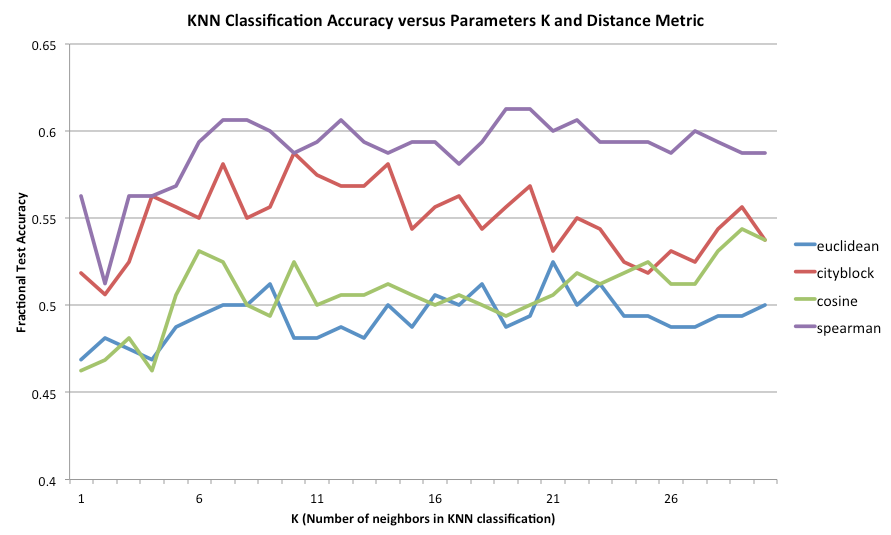
\includegraphics[width=\linewidth]{images/accuracy.png}
\caption{KNN Classification Accuracy versus Parameters K and Distance Metric}
\label{fig:accuracy}
\end{figure}

\end{document}

